\documentclass[a4paper]{article}
\usepackage{fancyhdr}
\usepackage[pdftex]{graphicx}
\usepackage{sidecap}
\usepackage{listings}
\usepackage{color}
\usepackage[export]{adjustbox}
\usepackage{subcaption}
\usepackage{graphicx}

\usepackage{hyperref}
\hypersetup{
    colorlinks=true,
    linkcolor=blue,
    filecolor=magenta, 
    urlcolor=cyan,
    bookmarks=true,
    pdfpagemode=FullScreen,
}
\usepackage{geometry}
 \geometry{
 a4paper,
 total={210mm,297mm},
 left=15mm,
 right=15mm,
 top=15mm,
 bottom=15mm,
 }

\usepackage{glossaries}


\makeglossaries
\newglossaryentry{FSM}
{
    name=FSM,
    description={Finite State Machine}
}

\definecolor{mygreen}{RGB}{25,172,0} % color values Red, Green, Blue
\definecolor{mylilas}{RGB}{170,55,241}
\definecolor{dkgreen}{rgb}{0,0.6,0}
\definecolor{gray}{rgb}{0.5,0.5,0.5}
\definecolor{mauve}{rgb}{0.58,0,0.82}

\pagestyle{fancy}
\fancyhf{}
\rhead{Vangjush Komini}
\lhead{KU Leuven}
\rfoot{Page \thepage}
\lfoot{Biomedical Data Processing part 2}


\lstset{inputpath=Code1}
\graphicspath{{Images1/}}

\include{Glossary}


\begin{titlepage}

\title{Assignment1\\\centerline{\textit{Subspace Signal Processing}} }

\author{
\href{mailto:vangjush.komini@uzleuven.be}{\textbf{Author:}Vangjush Komini}\\  \textit{r0612470} \\
\href{mailto:vangjush.komini@uzleuven.be}{vangjush.komini@uzleuven.be}\\
}





\end{titlepage}




\begin{document}



\maketitle
\begin{center}
\Large \href{https://onderwijsaanbod.kuleuven.be/syllabi/e/H06W1AE.htm#activetab=doelstellingen_idp41200}{Biomedical Data Processing, Part II Course}
\end{center}

\begin{figure}[!htbp]
\centering

\includegraphics[width=0.4\textwidth]{icon1.png}
\end{figure}



%\textbf{\Large Abstract:}
%Singular value decomposition SVD is a very powerful in linear signal processing. It offers an very accurate decomposition of the individual signals into orthogonal subspace where the mutual information is at the minimum level possible. Whereby any operation over distinct signals will eventually outcome promising results in terms of SNR and original signal distortion. Estimation of each parameters for each signal is another important benchmark for this modality. This is a rather optimisation problem where with a minimum variability bounded. Prior knowledge of any parameters contributes improves significantly this task. Moreover different types of reconstruction/enhancement aiming better signal-to-noise-ration proportionally to the alter of individual singular values. Multichannel data on the other hand are a very important hot topic 


%\footnote{This assignment contains 10 pages }

\section{Artefact removal}




\begin{figure}[!htbp]
\minipage{.5\textwidth}%
\centering
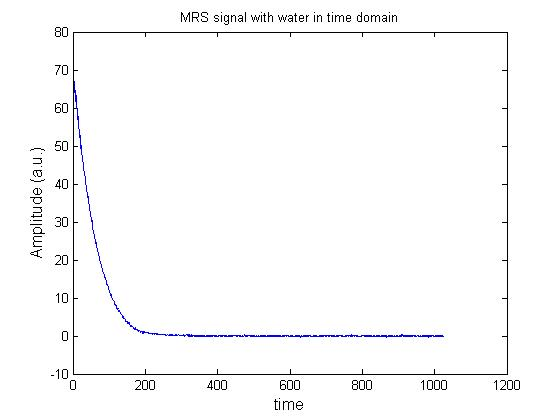
\includegraphics[width=.8\textwidth]{1.jpg}
\subcaption{Acquire signal in time domain}\label{1}
\endminipage\hfill
\minipage{.5\textwidth}%
\centering
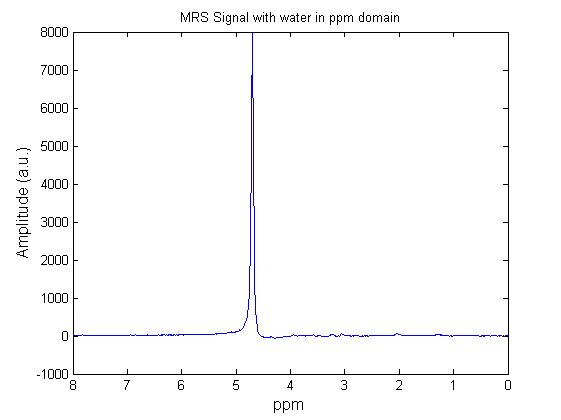
\includegraphics[width=.8\textwidth]{2.jpg}
\subcaption{Spectrum of the signal in ppm}\label{2}
\endminipage\hfill
\caption{The raw signal acquired from the MRS}
\end{figure}

 
Each component is exponentially damped complex-valued sinusoid of Lorentz type equation \ref{eq1}.


\begin{figure}[!htbp]
\minipage{.5\textwidth}%
\centering

\includegraphics[width=.8\textwidth]{3.jpg}
\subcaption{K component of the signal in time domain}\label{3}
\endminipage\hfill
\minipage{.5\textwidth}%
\centering
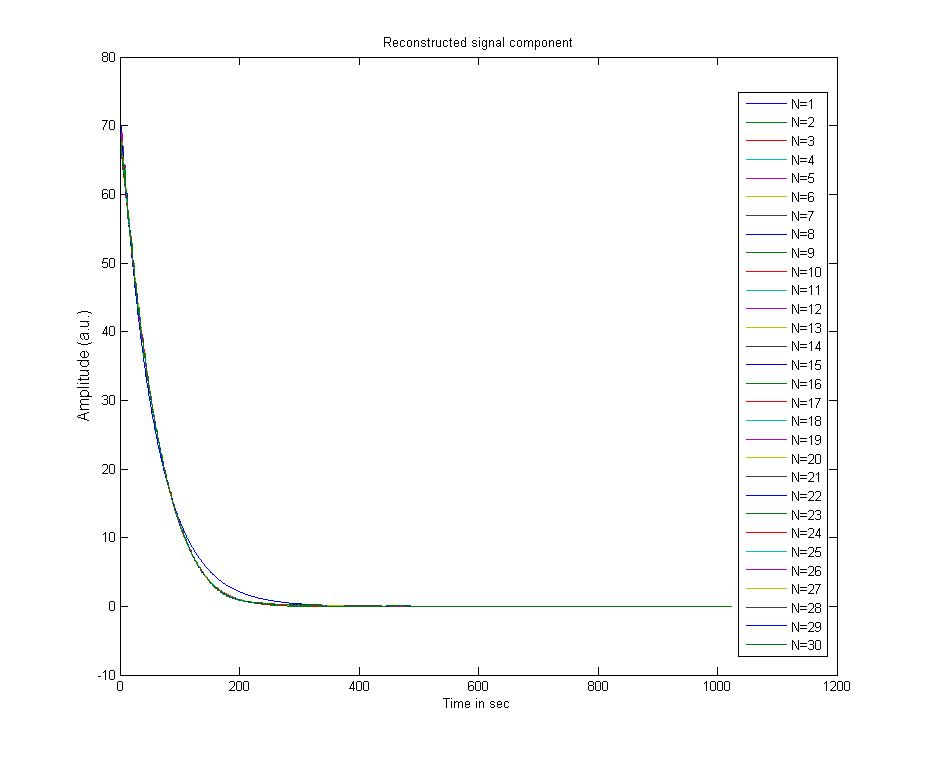
\includegraphics[width=.8\textwidth]{4.jpg}
\subcaption{Spectrum of the K component}\label{4}
\endminipage\hfill
\caption{Herein different metabolite component are extracted into individual part}
\end{figure}

The critical point is removing water is determination of components K which is related to the number of pics in the main spectrum. A reasonable number is required for a good SNR since underestimated K might omit the necessary pics to be suppressed. On the other hand a very large K could generate unwanted spectrum including noise component\cite{1}. 

\begin{equation}
SNR=20*\log\bigg\{\frac{OriginalSignal}{FilteredSignal-OriginalSignal}\bigg\}
\end{equation} 

In order estimate the number of needed components from the figure \ref{Nad1} there is a clear plot of the signal-to-noise ration versus the total number of components estimated. The SNR value theoretically should be as big as possible. This confirm that the extract signal has far more higher amplitude compare to the noise that was canceled out from the subspace filtering \cite{1}.

\begin{figure}[!htbp]
\centering
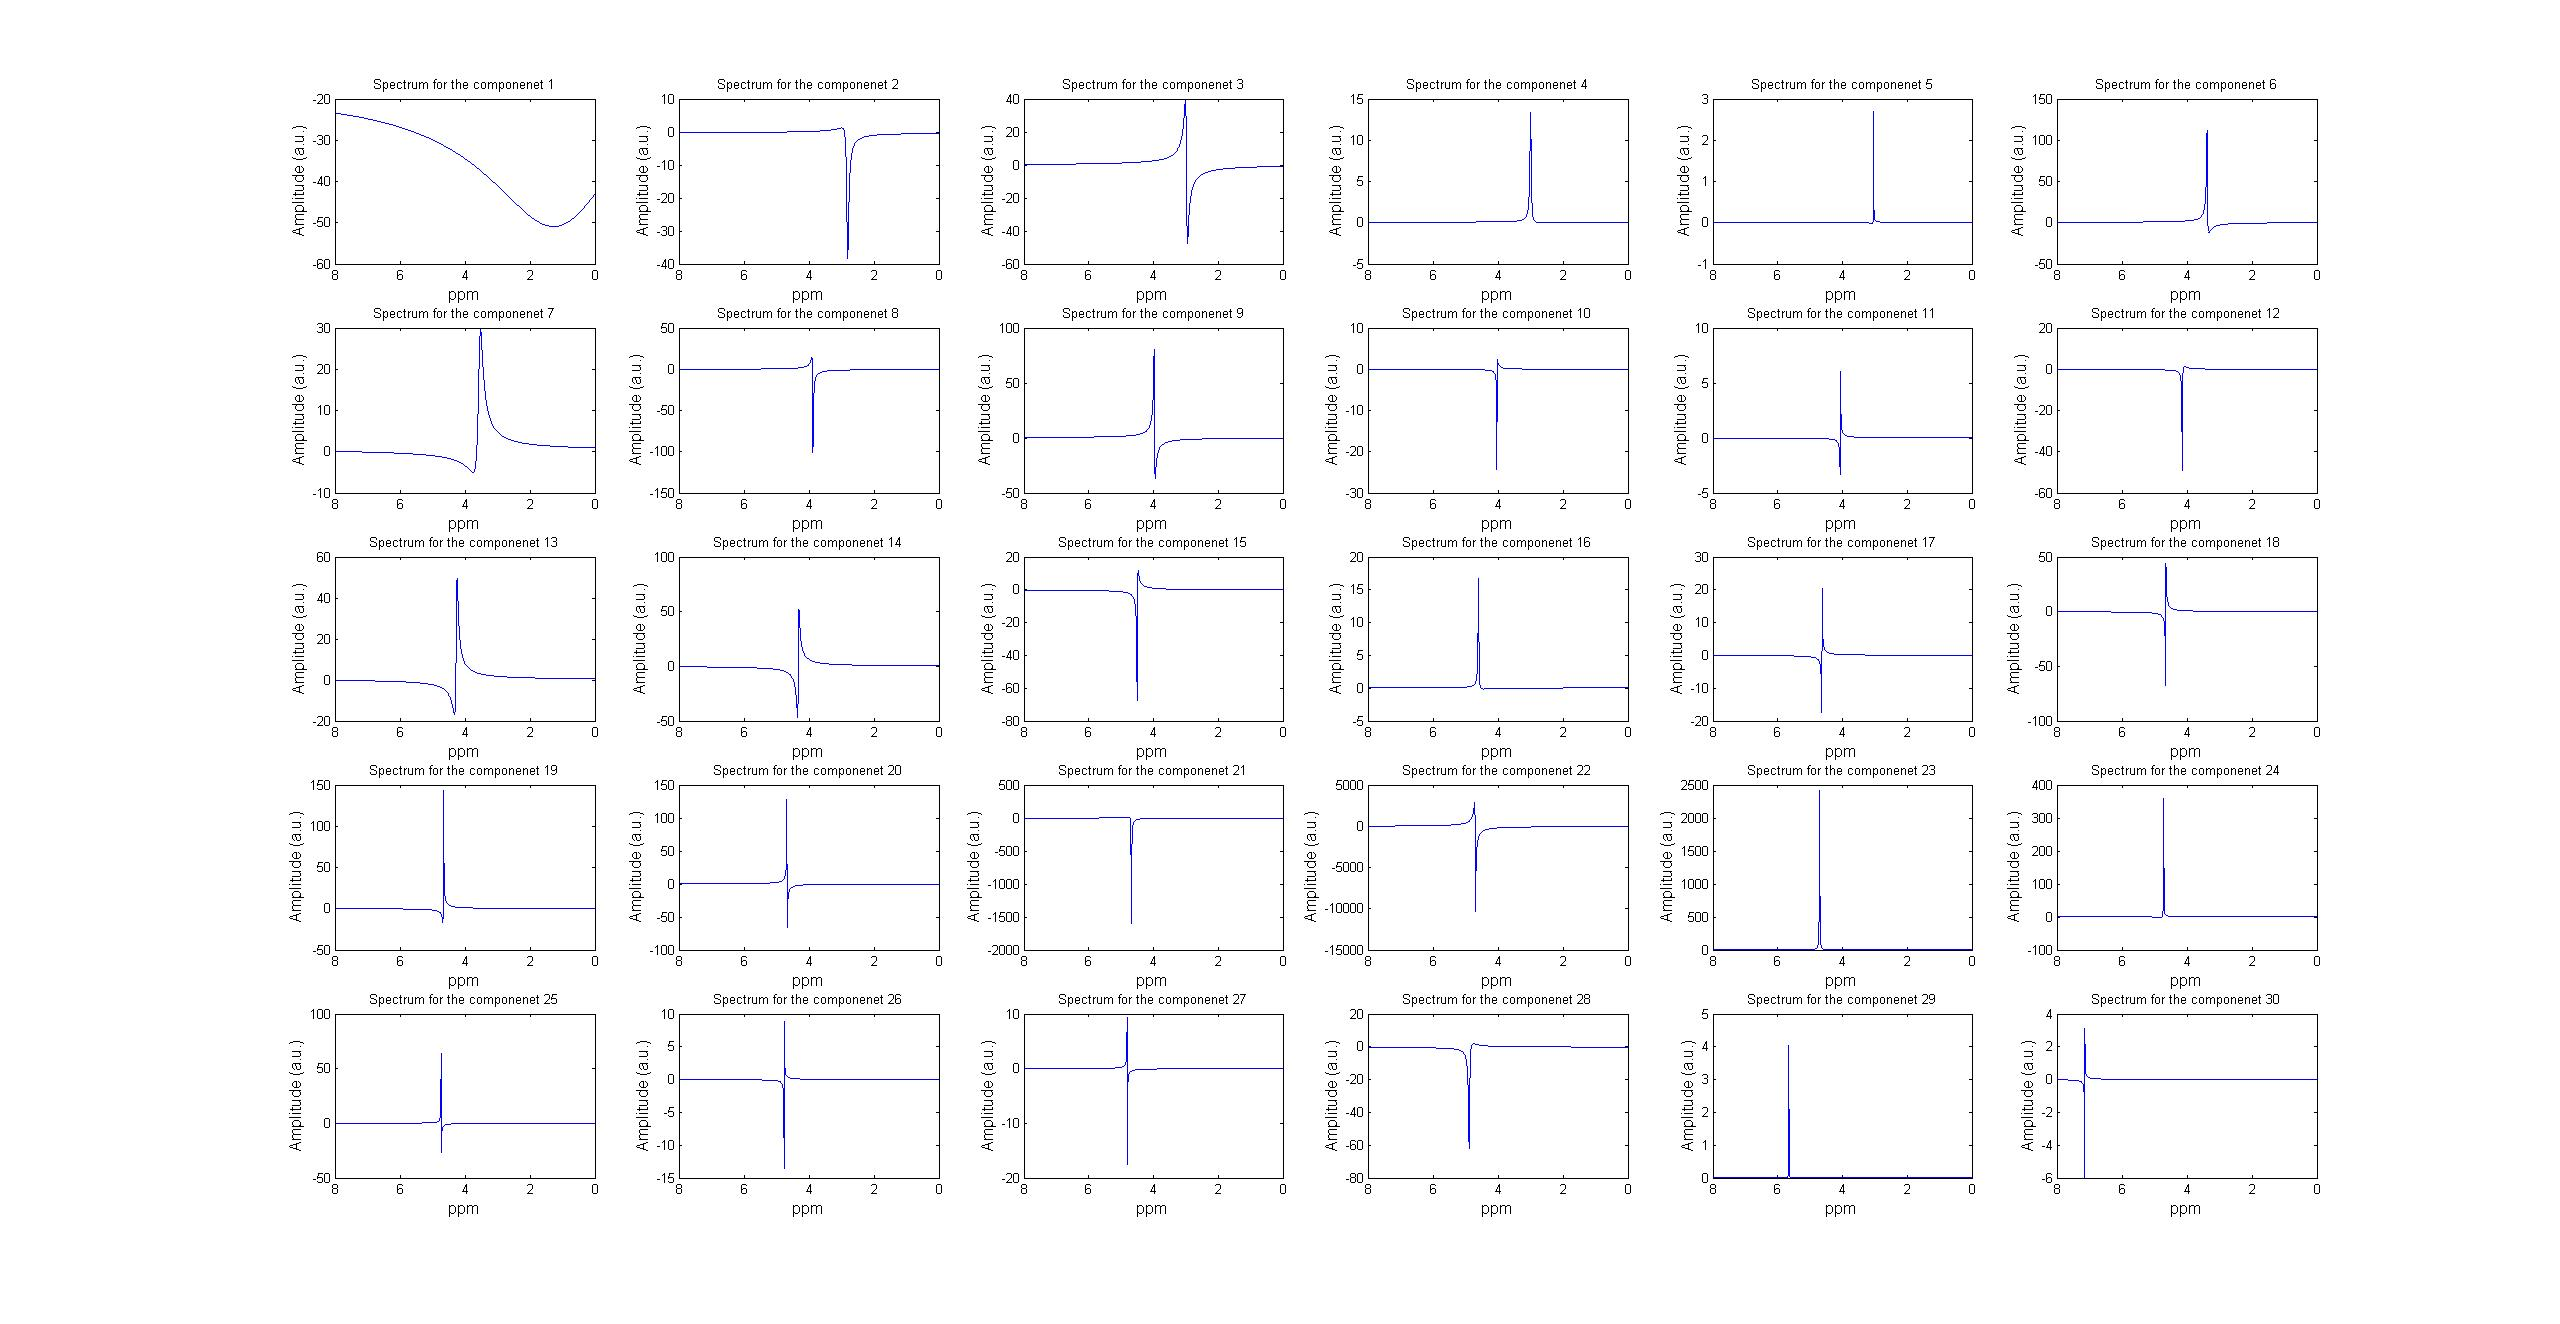
\includegraphics[width=1\textwidth]{5.jpg}
\caption{Spectrum components}\label{fig1}
\end{figure}

In the figure \ref{fig1} are the individual component where 30 is the model order. Herein it is notable that the central frequency increases as for at high order. After the suppression of the water components the spectrum of the filtered signal outcome has the pattern as in figure \ref{fig2}. Since the analysis was performed across different order the SNR estimation tends to stabilize at order higher than 19. In order to have the best cumulative estimation 30 as model order has been assigned throughout the following tasks. However it will be concluded into the third part of this session that for model lower than 30 the estimation is less accurate. Moreover the component with a central frequency sitting at higher than $4.7 ppm$ has to be suppressed. This component are displayed in both time and frequency domain respectively in figure \ref{fig5} and \ref{fig4} at \ref{S1A1}. 

The filtering has also been observed in model order. The results ate figure \ref{fig6} and \ref{fig7} indicate that high model order tends to include all possible peaks at the desired frequencies lower than $4.7ppm$. Another important fact is that watter peak is significantly high compare to the other metabolites. This is mainly due to the fact that watter composition in the body is $80\%$. Consequently by suppressing this peaks the relative scale in the plot will go down drastically and makes possible the other peaks to be very obvious fig \ref{fig2}. 


\begin{figure}[!htbp]

\minipage{.5\textwidth}%
\centering
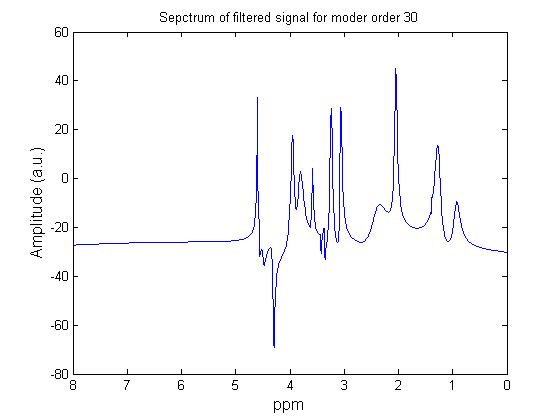
\includegraphics[width=1\textwidth]{8_1.jpg}
\subcaption{Spectrum Water filtered signal for model order 30}\label{fig2}
\endminipage\hfill
\minipage{.5\textwidth}%
\centering
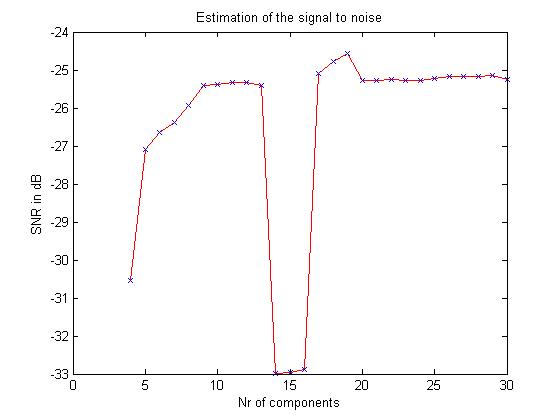
\includegraphics[width=1\textwidth]{11.jpg}
\subcaption{Signal-to-noise ration for different model order}\label{Nad1}
\endminipage\hfill
\caption{Cleaned signal from the water interference resided in the MRS spectrum fig \ref{1}}
\end{figure}

\newpage
\subsection{Comparison with classical filters}

Subspace filtering is a very powerful toolbox for noise removal composed of advantages and drawbacks compared to the other existing classical approaches such as spectral subtraction and Wiener filtering. Spectral extraction is restricted into a fixed FFT computational whereas SVD based topologies vary in computational time with the  Karhunen–Loève Transform data. In addition KLT transform $O(nm^2)$ is far more heavy in terms of computation compare to FFT $O(nlog(n))$ \cite{2}.

Moreover in this content subspace algorithm assume explicitly the order of the signal, or in other word the rank-deficient speech observation matrix. Whereas Wiener filtering does an implicit rank reduction based on a estimation of rank reduced correlation matrix \cite{2}.

Apart from the fft spectral approach, DCT is another candidate for signal enhancement yet it is far superior compare to the theoretical subspace filtering\cite{2}.

The benefits of using subspace filtering consist mainly on lower level of distortion when the signal is projected into the subspace with the minimum residue noise. Similarly the spectral extraction filter distort the desired signal but the residue level in this case is significantly higher resulting into low SNR level. Thus a moderation of signal distortion and nulling noisy component makes subspace algorithm superior to the classical filtering topologies \cite{3}.  

Another important aspect is the prior knowledge. This is an almost totally useless information for the classical filter. In the subspace case it increases the accuracy of parameter estimation and thus an higher SNR could be possible\cite{3}.

Differently from the classical filters, subspace approach efficiency depend significantly on the ability of the user to identify the accurately the characteristics of the underlying signal. The better the properties are defined the better the removal of the noises is performed\cite{5}. The other classical filters require no need of any additional visualization skills therefore are mostly applied in fully automated systems.

In order to consistently apply the subspace filtering, the signal has to be modelled into a clear analytical formulation. In some modalities this is not a very easy task consequently its application is restricted into very well known physical models.

Another fundamental issue with subspaces signal is that noise incorporated in the signal which needs to be reduced is considered white. In case of narrow band noises a pre-whitening step has to be applied before the the filtering itself takes place \cite{6}.



\section{Parameter estimation}

\begin{figure}[!htbp]
\minipage{.47\textwidth}%
\centering
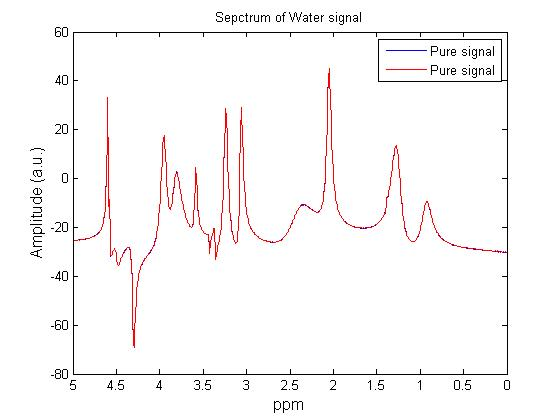
\includegraphics[width=1\textwidth]{35.jpg}
\subcaption{Spectrum of signals to be processed}
\endminipage\hfill
\minipage{.47\textwidth}%
\centering
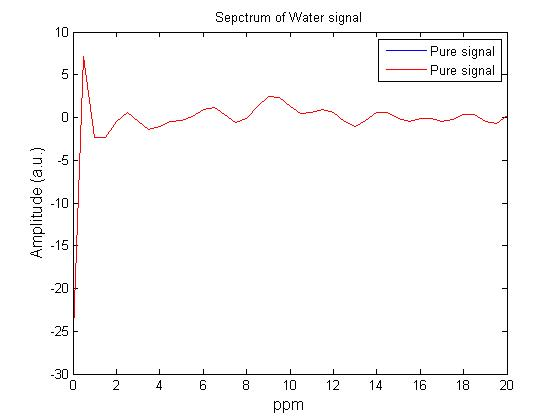
\includegraphics[width=1\textwidth]{36.jpg}
\subcaption{The signals to be processed in time domain}
\endminipage\hfill
\centering
\caption{The pure water filtered signal at model order 30 and the noisy signal coming from the superposition of the white Gaussian noise with mean zeros and the variance equal last 300 points of the water filtered signal}
\end{figure}



\begin{figure}[!htbp]
\minipage{.47\textwidth}%
\centering
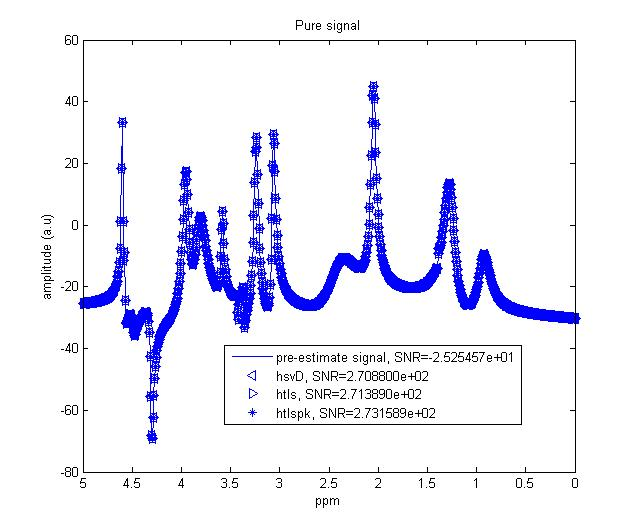
\includegraphics[width=1\textwidth]{22.jpg}
\subcaption{Reconstruction of noise free signal after hsvD, htls, htlspk estimation}\label{today1}
\endminipage\hfill
\minipage{.47\textwidth}%
\centering

\includegraphics[width=1\textwidth]{23.jpg}
\subcaption{Reconstruction of noisy signal after hsvD, htls, htlspk estimation}\label{today2}
\endminipage\hfill
\caption{Plot of the reconstructed spectrum for both the }
\end{figure}


\begin{figure}[!htbp]
\minipage{.47\textwidth}%
\centering
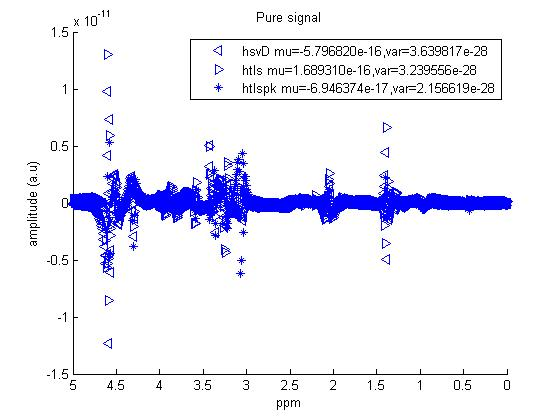
\includegraphics[width=1\textwidth]{24.jpg}
\subcaption{Residue of noise free signal after hsvD, htls, htlspk estimation}
\endminipage\hfill
\minipage{.47\textwidth}%
\centering
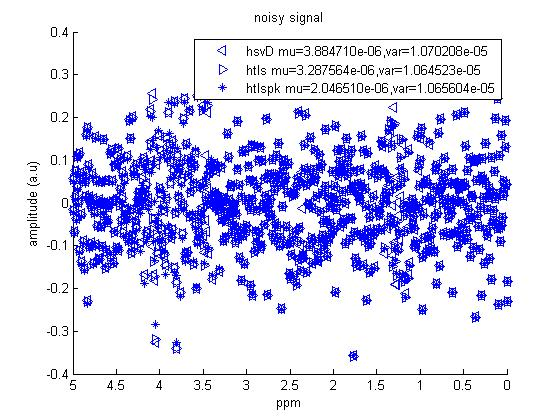
\includegraphics[width=1\textwidth]{25.jpg}
\subcaption{Residue of noisy signal after hsvD, htls, htlspk estimation}
\endminipage\hfill
\centering
\caption{The residue of both pure and noisy signals are included. This is computed as the difference between the input signal \textit{(pure or noisy)} and the outcome signal for respective method.}
\end{figure}

Using subspace methods for parameter estimation aims a very good fit between the reconstructed signal and the signal of interest. The accuracy of the method scales up, starting with the hsvD method moving into higher accuracy with htls. This is confirmed in both, SNR of the respective methods observed into the final signal and to the variance of the residue for respective signal. SNR tends to be higher contrary the variance tends to scale down, indicating a very good fit to the signal. In the figure \ref{today1} and \ref{today2} SNR values are bigger for the htls case compare to hsvD in both pure and noisy signal. In the work of \textbf{Chen et al 2011} it was possible to incorporate frequency and damping factor for the htls method. The result in the pure signal exhibit an improvement of the SNR compare to the both previous signals. Nevertheless it is still inferior compare to the htls without prior knowledge for the noisy signal case. This might outcome as a result of small inaccuracy of the prior knowledge which is incorporate subsequently arising into an less accurate results. 

Apart for the SNR  htlspkfd perform the best fit compare to both hsvd and htls in the pure signal case. Likewise, the fit tend to be less accurate in the noisy case from htlspkfd compare to htls, wherein under the same assumption. The prior values tend to be less accurate for the noisy signal consequently reflecting less accurate fit. 
However both SNR and the fit is much more accurate compare to the hsvd mode in both pure and noisy signal scenario. 
 

  

\newpage


























 \begin{table}[!htbp]
\centering
\caption{Frequency estimation \textbf{\textit{Hz}}}
\label{table:5}
\begin{tabular}{c c c c c c c c c c c c c c c c c c c c c c c c c c c c c c c } 
   \hline 

$Compo$&$HSVD$&$HTLS$&$HTLSPKFD$&$HSVD$&$HTLS$&$HTLSPKFD$\\
   \hline
$K$&$Pure signal$&$Pure signal$&$Pure signal$&$Noisy signal$&$Noisy signal$&$Noisy signal$\\
   \hline
   
   
   
   
$1$&$0.8987$&$ 0.9086$&$0.6562 $&$ 0.9081$&$ 0.9080$&$ 0.9080$\\
$2$&$0.8187$&$ 0.8071$&$ 0.5221$&$ 0.8317$&$ 0.8317$&$ 0.8321$\\
$3$&$0.6377$&$ 0.6377$&$ 0.4879$&$ 0.4122$&$ 0.4061$&$ 0.7914$\\
$4$&$0.5166$&$ 0.5166$&$-0.0128$&$ 0.2983$&$ 0.2983$&$ 0.2983$\\
$5$&$-0.0128$&$-0.0128$&$-0.0161$&$ 0.1575$&$ 0.1575$&$ 0.1575$\\
$6$&$-0.0161$&$-0.0161$&$-0.0268$&$ 0.0794$&$ 0.0794$&$ 0.0794$\\
$7$&$-0.0268$&$-0.0268$&$-0.0507$&$-0.0128$&$-0.0128$&$ -0.0128$\\
$8$&$-0.0507$&$-0.0507$&$-0.0929$&$-0.0161$&$-0.0161$&$ -0.0161$\\
$9$&$-0.0955$&$-0.0955$&$-0.0955$&$-0.0268$&$-0.0268$&$ -0.0268$\\
$10$&$-0.1118$&$-0.1118$&$-0.1118$&$-0.0507$&$-0.0507$&$ -0.0507$\\
$11$&$-0.1424$&$-0.1424$&$-0.1424$&$-0.0792$&$-0.0792$&$ -0.0789$\\
$12$&$-0.1624$&$-0.1624$&$-0.1624$&$-0.0955$&$-0.0955$&$ -0.0929$\\
$13$&$-0.1706$&$-0.1706$&$-0.1706$&$-0.1118$&$-0.1118$&$ -0.0955$\\
$14$&$-0.1864$&$-0.1864$&$-0.1864$&$-0.1424$&$-0.1424$&$ -0.1118$\\
$15$&$-0.2085$&$-0.2085$&$-0.2085$&$-0.1572$&$-0.1572$&$ -0.1423$\\
$16$&$-0.2195$&$-0.2100$&$-0.2126$&$-0.1624$&$-0.1624$&$ -0.1572$\\
$17$&$-0.2913$&$-0.2913$&$-0.2913$&$-0.1706$&$-0.1706$&$ -0.1624$\\
$18$&$-0.3029$&$-0.3026$&$-0.3013$&$-0.1864$&$-0.1864$&$ -0.1706$\\
$19$&$-0.3228$&$-0.3190$&$-0.3036$&$-0.2085$&$-0.2085$&$ -0.1864$\\
$20$&$-0.3386$&$-0.3386$&$-0.3386$&$-0.2914$&$-0.2914$&$ -0.2085$\\
$21$&$-0.3547$&$-0.3598$&$-0.3408$&$-0.2982$&$-0.2982$&$ -0.2914$\\
$22$&$-0.4229$&$-0.4229$&$-0.4195$&$-0.3386$&$-0.3386$&$ -0.2982$\\
$23$&$-0.4244$&$-0.4246$&$-0.4229$&$-0.4229$&$-0.4229$&$ -0.3386$\\
$24$&$-0.4306$&$-0.4313$&$-0.4237$&$-0.4356$&$-0.4358$&$ -0.4229$\\
$25$&$-0.4358$&$-0.4358$&$-0.4358$&$-0.4391$&$-0.4390$&$ -0.4359$\\
$26$&$-0.4391$&$-0.4391$&$-0.4391$&$-0.4810$&$-0.4810$&$ -0.4390$\\
$27$&$-0.4810$&$-0.4810$&$-0.4810$&$-0.8317$&$-0.8316$&$ -0.4810$\\
$28$&$-0.5441$&$-0.5441$&$-0.5434$&$-0.9080$&$-0.9080$&$ -0.8317$\\
$29$&$-0.6182$&$-0.6240$&$-0.5449$&$-0.9559$&$-0.9558$&$ -0.9080$\\
$30$&$-0.9561$&$-0.9561$&$-0.9561$&$-0.9830$&$-0.9770$&$ -0.9560$\\
   
   

    
     \hline 

\end{tabular}
\end{table}





 \begin{table}[!htbp]
\centering
\caption{Damping estimation \textbf{\textit{Hz}}}
\label{table:5}
\begin{tabular}{c c c c c c c c c c c c c c c c c c c c c c c c c c c c c c c } 
   \hline 
$Compo$&$HSVD$&$HTLS$&$HTLSPKFD$&$HSVD$&$HTLS$&$HTLSPKFD$\\
   \hline
$K$&$Pure signal$&$Pure signal$&$Pure signal$&$Noisy signal$&$Noisy signal$&$Noisy signal$\\
   \hline 
$1$  &$3.8888$&$ 3.8888$&$ 3.8888$&$ 3.8876$&$3.8875$&$3.8881$\\
$2$&$    1.8040$&$ 0.2089$&$ 0.5232$&$ 0.6610$&$ 0.1393$&$0.1394$\\
$3$ &$   0.7106$&$ 0.1812$&$ 0.1388$&$ 0.3541$&$ 0.0581$&$ 0.0730$\\
$4$  &$  0.4398$&$ 0.1387$&$ 0.0754$&$ 0.1394$&$ 0.0543$&$ 0.0581$\\
$5$&$    0.3966$&$ 0.0579$&$ 0.0729$&$ 0.0581$&$ 0.0504$&$ 0.0546$\\
$6$ &$   0.1991$&$ 0.0543$&$ 0.0580$&$ 0.0543$&$ 0.0326$&$ 0.0504$\\
$7$  &$  0.1387$&$ 0.0498$&$ 0.0543$&$ 0.0497$&$ 0.0298$&$ 0.0328$\\
$8$&$    0.1212$&$ 0.0371$&$ 0.0498$&$ 0.0363$&$0.0253$&$0.0297$\\
$9$ &$   0.0580$&$ 0.0325$&$ 0.0372$&$ 0.0326$&$ 0.0226$&$0.0253$\\
$ 10$ &$  0.0542$&$ 0.0253$&$ 0.0324$&$ 0.0253$&$ 0.0206$&$ 0.0226$\\
$11$&$    0.0498$&$ 0.0225$&$ 0.0253$&$ 0.0226$&$0.0172$&$0.0207$\\
$ 12$ &$  0.0421$&$ 0.0207$&$ 0.0226$&$ 0.0207$&$ 0.0149$&$0.0172$\\
$13$&$    0.0372$&$ 0.0181$&$ 0.0207$&$ 0.0172$&$ 0.0133$&$ 0.0149$\\
$14$ &$   0.0325$&$ 0.0171$&$ 0.0171$&$ 0.0149$&$ 0.0070$&$ 0.0133$\\
$ 15$ &$  0.0253$&$ 0.0148$&$ 0.0149$&$ 0.0133$&$ 0.0060$&$ 0.0070$\\
$16$&$    0.0226$&$ 0.0132$&$ 0.0133$&$0.0070$&$0.0058$&$0.0060$\\
$17$ &$   0.0207$&$ 0.0115$&$ 0.0071$&$ 0.0060$&$ 0.0036$&$0.0058$\\
$ 18$ &$  0.0172$&$ 0.0095$&$ 0.0061$&$ 0.0058$&$ 0.0024$&$ 0.0034$\\
$19$&$    0.0149$&$ 0.0070$&$ 0.0056$&$ 0.0024$&$ 0.0014$&$ 0.0024$\\
$20$&$   0.0133$&$ 0.0060$&$ 0.0036$&$ 0.0022$&$ 0.0011$&$ 0.0014$\\
$21$ &$  0.0071$&$ 0.0057$&$ 0.0026$&$ 0.0018$&$ 0.0010$&$ 0.0010$\\
$22$&$    0.0061$&$ 0.0024$&$0.0023$&$0.0016$&$0.0007$&$0.0007$\\
$23$ &$   0.0060$&$ 0.0015$&$ 0.0013$&$0.0015$&$-0.0001$&$-0.0002$\\
$24$  &$  0.0057$&$ 0.0014$&$ 0.0011$&$0.0014$&$-0.0002$&$-0.0002$\\
$25$   &$ 0.0057$&$ 0.0009$&$ 0.0006$&$0.0014$&$-0.0002$&$-0.0002$\\
$26$    &$0.0024$&$ 0.0007$&$ 0.0005$&$0.0012$&$-0.0002$&$-0.0002$\\
$27$&$    0.0014$&$ 0.0001$&$ 0.0000$&$0.0008$&$-0.0003$&$-0.0003$\\
$28$&$    0.0011$&$ -0.0001$&$-0.0003$&$0.0003$&$-0.0004$&$-0.0004$\\
$29$ &$  -0.0029$&$-0.0035$&$-0.0011$&$0.0002$&$-0.0013$&$-0.0016$\\
$ 30$ &$ -0.0031$&$-0.0035$&$-0.0031$&$-0.0003$&$-0.0016$&$-0.0016$\\
    \hline 

\end{tabular}
\end{table}


 \begin{table}[!htbp]
\centering
\caption{Amplitude estimation \textbf{\textit{a.u}}}
\label{table:5}
\begin{tabular}{c c c c c c c c c c c c c c c c c c c c c c c c c c c c c c c } 
   \hline 
$Compo$&$HSVD$&$HTLS$&$HTLSPKFD$&$HSVD$&$HTLS$&$HTLSPKFD$\\
   \hline
$K$&$Pure signal$&$Pure signal$&$Pure signal$&$Noisy signal$&$Noisy signal$&$Noisy signal$\\
   \hline 
$1   $&$32.6329$&$32.6329$&$32.6329$&$32.6298$&$32.6280$&$32.6303$\\
$2   $ &$1.1981$&$ 1.1981$&$ 1.1981$&$1.2022$&$1.2014$&$1.2020$\\
$3$&$    1.0859$&$ 1.0859$&$ 1.0859$&$1.0798$&$1.1177$&$ 1.1213$\\
$4$ &$   0.9033$&$ 0.9033$&$ 0.9033$&$ 0.9037$&$0.9034$&$0.9120$\\
$5$  &$  0.8092$&$ 0.8092$&$ 0.8092$&$ 0.8112$&$ 0.8112$&$0.8266$\\
$6$&$    0.8086$&$ 0.8086$&$ 0.8086$&$ 0.8073$&$ 0.8074$&$ 0.8074$\\
$7$ &$   0.6667$&$ 0.6667$&$ 0.6667$&$ 0.6661$&$ 0.6661$&$ 0.6664$\\
$8$  &$  0.5733$&$ 0.5732$&$ 0.5733$&$ 0.5737$&$ 0.5737$&$ 0.5738$\\
$9$   &$ 0.5072$&$ 0.5072$&$ 0.5072$&$ 0.5071$&$ 0.5070$&$ 0.5072$\\
$10$    &$0.3205$&$ 0.3205$&$ 0.3205$&$ 0.3201$&$ 0.3201$&$ 0.3204$\\
$11 $   0&$.2034$&$ 0.2035$&$ 0.2035$&$ 0.2034$&$ 0.2034$&$ 0.2034$\\
$12 $   0.&$1825$&$ 0.1825$&$ 0.1825$&$ 0.1826$&$ 0.1826$&$ 0.1828$\\
$13$&$    0.1245$&$ 0.1245$&$ 0.1245$&$ 0.1205$&$ 0.0930$&$ 0.0931$\\
$14$ &$   0.0932$&$ 0.0931$&$ 0.0931$&$ 0.0930$&$ 0.0726$&$ 0.0735$\\
$15$  &$  0.0653$&$ 0.0653$&$ 0.0653$&$ 0.0657$&$ 0.0657$&$ 0.0656$\\
$16$&$    0.0439$&$ 0.0439$&$ 0.0439$&$ 0.0432$&$ 0.0432$&$ 0.0432$\\
$17$ &$   0.0192$&$ 0.0191$&$ 0.0192$&$ 0.0190$&$ 0.0189$&$ 0.0216$\\
$18$  &$  0.0099$&$ 0.0098$&$ 0.0099$&$ 0.0100$&$ 0.0100$&$ 0.0189$\\
$19$&$    0.0000$&$ -0.0001$&$ 0.0000$&$0.0020$&$ 0.0003$&$ 0.0101$\\
$20$ &$   0.0000$&$ 0.0000$&$-0.0001$&$0.0015$&$0.0003$&$0.0003$\\
$21$  &$  0.0000$&$ -0.0001$&$ 0.0000$&$0.0004$&$  0.0003$&$0.0002$\\
$22$&$    0.0000$&$ 0.0000$&$0.0000$&$0.0003$&$0.0002$&$0.0001$\\
$23$ &$   0.0000$&$ 0.0000$&$ 0.0000$&$0.0002$&$0.0001$&$0.0001$\\
$24$  &$  0.0000$&$ 0.0000$&$ 0.0000$&$ 0.0002$&$0.0001$&$0.0001$\\
$25$   &$ 0.0000$&$ -0.0001$&$ 0.0000$&$0.0002$&$ 0.0001$&$0.0001$\\
$26$    &$0.0000$&$ 0.0000$&$0.0000$&$0.0002$&$0.0001$&$0.0001$\\
$27$&$  0.0000$&$ 0.0000$&$ 0.0000$&$0.0002$&$0.0001$&$0.0001$\\
$28$&$    -0.0001$&$ -0.0001$&$0.0000$&$0.0002$&$0.0001$&$0.0001$\\
$29$   &$ -0.0001$&$0.0000$&$0.0000$&$0.0001$&$0.0000$&$0.0001$\\
$30$    &$-0.0001$&$-0.0001$&$0.0000$&$0.0000$&$0.0000$&$0.0000$\\
     \hline 

\end{tabular}
\end{table}



 \begin{table}[!htbp]
\centering
\caption{Phase estimation \textbf{\textit{Deg}}}
\label{table:5}
\begin{tabular}{c c c c c c c c c c c c c c c c c c c c c c c c c c c c c c c } 
   \hline 

$Compo$&$HSVD$&$HTLS$&$HTLSPKFD$&$HSVD$&$HTLS$&$HTLSPKFD$\\
   \hline
$K$&$Pure signal$&$Pure signal$&$Pure signal$&$Noisy signal$&$Noisy signal$&$Noisy signal$\\
   \hline 
$1$&$  353.0457$&$353.0457$&$353.9060$&$353.3338$&$353.0316$&$353.0277$\\
$2$ &$ 352.5020$&$352.5020$&$353.0457$&$353.0305$&$352.5485$&$352.5421$\\
$3$ &$ 342.7687$&$342.7687$&$352.5020$&$352.5437$&$342.7033$&$342.6403$\\
$4$  &$342.0433$&$342.0433$&$345.1340$&$342.6973$&$341.9824$&$341.9757$\\
$5$&$  329.1565$&$329.1565$&$342.7687$&$342.0679$&$329.1524$&$329.1508$\\
$6$ &$ 325.6619$&$325.6619$&$342.0433$&$329.1519$&$325.5254$&$325.5798$\\
$7$  &$313.3449$&$313.3449$&$341.2040$&$325.5312$&$313.2785$&$313.3143$\\
$8$&$  311.4413$&$282.7090$&$329.1565$&$313.2660$&$308.6737$&$309.0136$\\
$9$ &$ 307.8060$&$259.6805$&$325.6619$&$304.4009$&$304.2548$&$303.4103$\\
$10$  &$282.7090$&$256.9107$&$313.3450$&$282.7573$&$282.9388$&$282.9014$\\
$11$&$  279.4737$&$249.8693$&$296.2705$&$277.5808$&$275.9693$&$254.9584$\\
$12$ &$ 259.8489$&$227.0606$&$282.7090$&$272.2716$&$256.0013$&$249.6786$\\
$13$  &$238.4413$&$185.6412$&$243.8925$&$265.5952$&$204.8138$&$218.4549$\\
$14$&$  234.6404$&$149.5597$&$185.6412$&$212.2177$&$185.6322$&$185.6365$\\
$15$ &$ 185.6411$&$148.4096$&$168.8839$&$185.6279$&$150.1872$&$177.1757$\\
$16$  &$170.1475$&$126.3778$&$161.5672$&$150.2351$&$148.4314$&$162.9075$\\
$17$  &$149.5597$&$122.6237$&$158.7715$&$148.4255$&$147.6220$&$150.1472$\\
$18$  &$148.4096$&$119.5757$&$149.5597$&$140.8382$&$141.7136$&$148.4846$\\
$19$&$  119.5757$&$100.6838$&$148.4096$&$119.7685$&$122.7716$&$125.3330$\\
$20 $&$ 100.6838$&$97.9307$&$119.5757$&$98.5117$&$119.7707$&$120.0598$\\
$21 $ &$ 98.8727$&$74.9523$&$101.4028$&$98.4081$&$98.3968$&$98.3028$\\
$22$&$   97.9306$&$71.4598$&$100.6838$&$85.3232$&$98.3468$&$ 61.1008$\\
$23$ &$  91.5578$&$48.6633$&$97.9307$&$77.8430$&$50.5836$&$52.7016$\\
$24$  &$ 90.6754$&$29.7034$&$80.2124$&$49.8303$&$49.3632$&$49.8074$\\
$25$&$   63.3129$&$16.1521$&$48.6633$&$49.0087$&$47.8449$&$47.8806$\\
$26$ &$  51.2416$&$14.2335$&$29.7034$&$47.8570$&$36.5071$&$46.9110$\\
$27 $ &$ 48.6633$&$13.6347$&$14.2336$&$29.8902$&$29.8965$&$29.8477$\\
$28 $  &$29.7034$&$ 7.2483$&$ 4.7676$&$14.4915$&$19.1006$&$17.1431$\\
$29 $  &$14.2336$&$ 6.9159$&$ 3.9155$&$13.7611$&$17.1397$&$16.3458$\\
$30 $   &$4.7676$&$ 4.7675$&$ 3.1099$&$4.7621$&$4.7517$&$5.1473$\\
   \hline 

\end{tabular}
\end{table}  
    
    
      
\newpage
\subsection{Subspace methods for parameter estimation}
 Parameter estimation is possible via either via subspace methods, or via optimization methods.
 
 Subspace methods employs least square estimation technique for the estimation of the parameters. This is an optimization technique where the real intended value is never reached in real scenario. The lower bound of this bias estimation is outcomed from Cramer-Rao criteria. The ambiguity of this estimation increases with the number of the unknown parameter and this is even conformed from the Fisher information matrix. 
 
 
Even tough very hard to be done, it is possible to incorporate prior knowledge on the estimation this will increase the accuracy of the parameter estimation \cite{7}. The more prior knowledge we have the more accurate the estimation will be. Different types of prior knowledge has a totally different approach for their incorporation where in most of the cases is never straight forward\cite{8}.

Contrary to the optimization based methods subspace methods don't require any iterative estimation consequently the complexity in this case far better. Moreover the estimation requires no cost function to be modeled where its importance is mostly related to the number of steps towards the best result.

Subspace methods does not ensure the best estimation possible however it ensures that there is not local minimum reached, which in the optimization case this could be possible when the method does not explore the candidates globally. However via prior knowledge the CR bound is approached quite significantly\cite{7}.

The user capability to initialize the parameters of the subspace methods is very important. In case of MRS signal the number of peaks is an visual estimated. This restricted the method from being fully automatized. 

Subspace methods are very good candidate for the parameter estimation of closely spaced sinusoid thereby making them excellent method for metabolite detection in MRS \cite{9}.  

Subspace methods are very robust estimation, meaning that they will claim a good result out in best scenario whereas in the optimization method, some internal error could occur during the computation of the cost function\cite{9}.

Furthermore, subspace methods are capable for parameter estimation of multiple different signals at the same time via the extension of the existing HTLS based algorithms\cite{10}. Consequently big data could be processed simultaneously instead of a iteration over single signal in the optimization case.

Last but not least the same estimation over the same values is not ensured via subspace methods for parameter estimation. 



\section{Noise removal}


\begin{figure}[!htbp]
\minipage{.47\textwidth}%
\centering
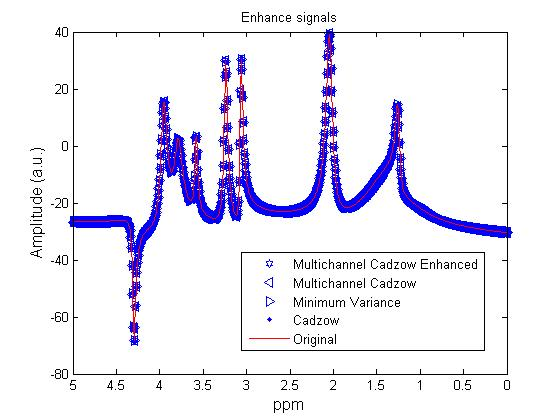
\includegraphics[width=1\textwidth]{27.jpg}
\subcaption{Original signal and its respective enhancement after Cadzow, Minimum variance, Multichannel Cadzow, and Enhanced Multichannel Cadzow}
\endminipage\hfill
\minipage{.47\textwidth}%
\centering
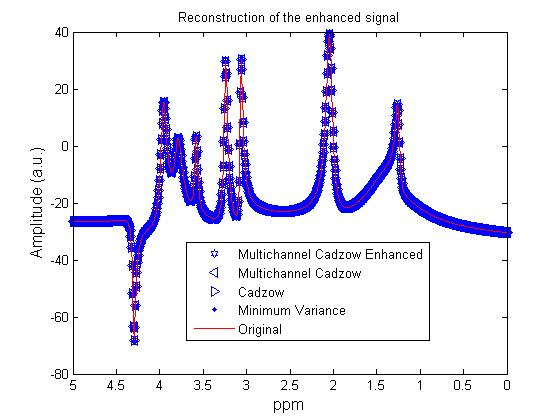
\includegraphics[width=1\textwidth]{28.jpg}
\subcaption{Original signal and its respective estimation after Cadzow, Minimum variance, Multichannel Cadzow, and Enhanced Multichannel Cadzow enhancement}
\endminipage\hfill
\caption{Enhancement of the signal employing both single channel and multichannel approach}
\end{figure}

Hereby different enhancement techniques are being investigated. Starting with the Cadzow technique which consist of a simple truncation of the singular values decomposition method. Meaning that the low singular values (low level of information) is canceled out due to its inferior contribution to the spectrum of interest.

Minimum variance in addition in addition to truncation tries to decrease the residue of the singular values with an arbitrary value as:

\begin{equation}
\sigma_{i}=\sigma_{i}-\sigma_{r}
\end{equation}

where $\sigma_{r}$ in our implementation consist of the average of the dropped singular values dropped by the truncation\cite{11}. This could also be the smalles value of the singuar matrix which has been used in other implementation\cite{2}. This method indicates a very small SNR improvement. This far it was only taken into the consideration the single channel enhancement technique. When neighbouring of the main voxels with the distance of 3x3 voxel are taken into account an significant improvement of the signal to noise ration has been investigated. In the figure \ref{figtoda1} there is an overview of the voxel of interest together with its 9x9 neighbours. In the first implementation, 9 signals are taken into a neighbourhood of 3x3 voxels where the main voxel is the region of the interest. Then each of the signal is reshaped into an Hankel matrix thus 9 matrices in total. These matrices are then merged horizontally one by one to creating a array of matrices and the final matrix consist of the signal to be proceeded. SVD is computed from this matrix which is a very heavy computation. A model order of 30 has been incorporated into this computation, meaning that truncation after the SVD will take only the first 30 singular values. After the truncation the matrix of our interest which contain the signal of the main voxel is picked up and average along the anti-diagonal. The result is another Hankel matrix where after reshaping the matrix into the original signal dimension and much higher SNR has been observed. Some important remarks are: ordering of the signals when the Hankel matrices are merged does not influence the result \cite{14}. The model order is fixed and there is only one step of performed for this estimation. 

However the multichannel method is further improved by taking different order of the model and by taking different distance of the neighbours. Starting with a 3x3 neighbours and moving into 5x5,7x7, and 9x9. This is first performed along the horizontal and vertical neighbours then along the diagonal and anti-diagonal neighbours. Whereas due to the memory complexity and limited resources it was not possible to run with full neighbourhoods at scale higher than 5x5. It has been observed that SNR tends to decay for higher neighbourhood for lower model order. Thus it was decided to not run the full neighbourhood model since from the 5x5 SNR is lower than 3x3. Moreover this goes the same for the other two neigbhourhooding.  


Starting with the water filter signal where its SNR is \textbf{\textit{$-25.2546 dB$}} Cadzow outcomes an significant improvement of the SNR up to $3.7264 dB$. Minimum variance implementation tends to be slightly higher compare to Cadzow nevertheless is still an improvement with is translated into lower level of noise. Further more the noise suppression is far higher in the multichannel case where $3x3$ voxel will yield an SNR of $39.5513$ whereas $5x5$ voxel case will yield a slightly lower SNR of $38.5198 dB$. Since the SNR decays as the number of neighbours voxels increases SNR tends to decays thus there was no encouragement in testing the ordinary Multichannel Cadzow despite its memory and time complexity which is technically NP. Since time complexity is a more desirable  compare to memory complexity.  Even though both are bad scenario memory requires physical resources whereas time could be achieved by just waiting. 
The best performance is achieved with vertically and horizontally neighbours at order of 22 with 3x3 voxels with a SNR of \textbf{\textit{$40.1137 dB$}}. This method however performs better compare to the diagonal and anti-diagonal version   respectively to model order and voxels range. This could be concluded from the table \ref{niceday} and table \ref{niceday1}. Further more for the cases of 3x3 and 5x5 range the generic Multichannel Cadzow tends to be higher compare to the anti-diagonal case however is still inferior to the horizontal and vertical case.


%%%%%%%%%%%%%%%%%%%%%%%%%%%%%%%%%%%%%%%%%%%%%%%%%%%%%%%%%%%%%%%%%%%%%%%%%%%%%%%%%%%%%%%%%%%%%%%%%%%%%%%%%%%%%%%%%%%%%%%%%%%%%%%%%%%%%%%%%%%%%%%%%%%%%%%%%%%%%%%%%%%%%%%%%%%%%%%%%%%%%%%%%%%%


\begin{table}[!htbp]
\centering
\caption{Signal to noise values for the anti diagonal and diagonal neighbours at $dB$ level. Different model are tested further more using different neighbouring range}\label{niceday}
\label{table:55}
\begin{tabular}{c c c c c c c c c c c c c c c c c}
  \hline  
$K$&$30$&$29$&$28$&$27$&$26$&$25$&$24$&$23$&$22$&$21$&$20$\\
  \hline  
$3x3$&$36.2700$&$37.7028$&$36.0013$&$35.8031$&$35.4027$&$35.7358$&$35.7531$&$35.4922$&$37.1925$&$37.6473$&$37.6407$\\
$5x5$&$36.4102$&$37.7397$&$36.0068$&$35.9564$&$35.3598$&$35.7904$&$35.6169$&$35.7460$&$37.1497$&$37.6843$&$37.7884$\\
$7x7$&$36.1939$&$37.7153$&$35.9040$&$36.0002$&$35.3396$&$35.8426$&$35.5035$&$35.7533$&$37.1429$&$37.6568$&$37.7309$\\
$9x9$&$35.8524$&$36.9298$&$35.7412$&$36.1220$&$35.3127$&$35.9223$&$35.5232$&$35.7155$&$37.1599$&$37.8243$&$37.5072$\\
  \hline  
\end{tabular}
\end{table}  
  
  
  \begin{table}[!htbp]
\centering
\caption{Signal to noise values for the  vertical and horizontal neighbours at $dB$ level. Different model are tested further more using different neighbouring range}\label{niceday1}
\label{table:55}
\begin{tabular}{c c c c c c c c c c c c c c c c c} 
  \hline  
$K$&$30$&$29$&$28$&$27$&$26$&$25$&$24$&$23$&$22$&$21$&$20$\\
  \hline  
$3x3$&$40.0829$&$39.1976$&$37.6684$&$37.0776$&$36.1116$&$37.5342$&$35.8595$&$34.8111$&\textbf{\textit{$40.1137$}}&$38.0277$&$37.6797$\\
$5x5$&$38.1118$&$36.5473$&$37.0211$&$36.7936$&$35.2903$&$35.2727$&$34.9380$&$34.8007$&$37.4030$&$36.6630$&$33.8714$\\
$7x7$&$36.7022$&$36.5759$&$37.0355$&$36.5761$&$35.0747$&$35.1001$&$34.9214$&$34.7472$&$37.4039$&$36.6613$&$33.8988$\\
$9x9$&$36.9532$&$36.6120$&$37.0117$&$36.4066$&$35.0171$&$35.1019$&$34.8839$&$34.7718$&$37.3859$&$36.5159$&$33.9277$\\
 \hline
\end{tabular}
\end{table}



 \begin{table}[!htbp]
\centering
\caption{Frequency estimation \textbf{\textit{Hz}}}
\label{table:5}
\begin{tabular}{c c c c c c c c c c c c c c c c c c c c c c c c c c c c c c c } 
   \hline 
$Signals$&$Pure$&$Cdz$&$MinVar$&$MultiCh$&$OptiMultiCha$\\
   \hline 

$1$&$ 0.9079$&$ 0.9127$&$ 0.8988$&$-0.0129$&$-0.0127$\\
$2$&$ 0.8004$&$ 0.7810$&$ 0.6782$&$-0.0151$&$-0.0129$\\
$3$&$ 0.6815$&$ 0.7116$&$ 0.2674$&$-0.0160$&$-0.0162$\\
$4$&$ 0.2310$&$ 0.2280$&$-0.0128$&$-0.0257$&$-0.0507$\\
$5$&$-0.0128$&$-0.0128$&$-0.0508$&$-0.0506$&$-0.0630$\\
$6$&$-0.0508$&$-0.0508$&$-0.0949$&$-0.0700$&$-0.0951$\\
$7$&$-0.0949$&$-0.0949$&$-0.0954$&$-0.0954$&$-0.1143$\\
$8$&$-0.0954$&$-0.0954$&$-0.1168$&$-0.1119$&$-0.1148$\\
$9$&$-0.1168$&$-0.1168$&$-0.1429$&$-0.1424$&$-0.1427$\\
$10$&$-0.1429$&$-0.1429$&$-0.1645$&$-0.1623$&$-0.1632$\\
$11$&$-0.1645$&$-0.1645$&$-0.1863$&$-0.1679$&$-0.1634$\\
$12$&$-0.1863$&$-0.1863$&$-0.1903$&$-0.1704$&$-0.1636$\\
$13$&$-0.2085$&$-0.2082$&$-0.2085$&$-0.1731$&$-0.1651$\\
$14$&$-0.2166$&$-0.2085$&$-0.3137$&$-0.1864$&$-0.1863$\\
$15$&$-0.3144$&$-0.3169$&$-0.3396$&$-0.2085$&$-0.2085$\\
$16$&$-0.3239$&$-0.3396$&$-0.3441$&$-0.2920$&$-0.2653$\\
$17$&$-0.3396$&$-0.3578$&$-0.4273$&$-0.3385$&$-0.3396$\\
$18$&$-0.3825$&$-0.4273$&$-0.4409$&$-0.4226$&$-0.3956$\\
$19$&$-0.4273$&$-0.4409$&$-0.4576$&$-0.4234$&$-0.4229$\\
$20$&$-0.4409$&$-0.4972$&$-0.4647$&$-0.4387$&$-0.4406$\\
$21$&$-0.6682$&$-0.9445$&$-0.9371$&$-0.4818$&$-0.4776$\\
$22$&$-0.9445$&$-0.9996$&$-0.9445$&$-0.9535$&$-0.9429$\\
     \hline 

\end{tabular}
\end{table}

 \begin{table}[!htbp]
\centering
\caption{Damping estimation \textbf{\textit{Hz}}}
\label{table:5}
\begin{tabular}{c c c c c c c c c c c c c c c c c c c c c c c c c c c c c c c } 
   \hline 
$Signals$&$Pure$&$Cdz$&$MinVar$&$MultiCh$&$OptiMultiCha$\\
   \hline 
$1$&$ 4.0342$&$ 4.0342$&$ 4.1211$&$ 3.9398$&$ 3.9937$\\
$2$&$ 0.5761$&$ 1.2324$&$ 4.0342$&$ 0.1416$&$ 0.3137$\\
$3$&$ 0.5179$&$ 0.8633$&$ 0.7609$&$ 0.0689$&$ 0.2699$\\
$4$&$ 0.3748$&$ 0.7635$&$ 0.4569$&$ 0.0610$&$ 0.1916$\\
$5$&$ 0.2642$&$ 0.3748$&$ 0.3748$&$ 0.0548$&$ 0.1731$\\
$6$&$ 0.2633$&$ 0.2633$&$ 0.2633$&$ 0.0539$&$ 0.1129$\\
$7$&$ 0.1784$&$ 0.2361$&$ 0.1900$&$ 0.0322$&$ 0.0823$\\
$8$&$ 0.0829$&$ 0.1674$&$ 0.1446$&$ 0.0259$&$ 0.0762$\\
$9$&$ 0.0700$&$ 0.0700$&$ 0.1082$&$ 0.0253$&$ 0.0613$\\
$10$&$ 0.0407$&$ 0.0617$&$ 0.1012$&$ 0.0226$&$ 0.0357$\\
$11$&$ 0.0378$&$ 0.0497$&$ 0.0740$&$ 0.0172$&$ 0.0318$\\
$12$&$ 0.0355$&$ 0.0396$&$ 0.0700$&$ 0.0146$&$ 0.0262$\\
$13$&$ 0.0351$&$ 0.0355$&$ 0.0477$&$ 0.0135$&$ 0.0202$\\
$14$&$ 0.0303$&$ 0.0303$&$ 0.0355$&$ 0.0085$&$ 0.0160$\\
$15$&$ 0.0246$&$ 0.0246$&$ 0.0303$&$ 0.0077$&$ 0.0155$\\
$16$&$ 0.0205$&$ 0.0202$&$ 0.0246$&$ 0.0069$&$ 0.0152$\\
$17$&$ 0.0202$&$ 0.0174$&$ 0.0202$&$ 0.0053$&$ 0.0146$\\
$18$&$ 0.0174$&$ 0.0153$&$ 0.0174$&$ 0.0052$&$ 0.0144$\\
$19$&$ 0.0153$&$ 0.0149$&$ 0.0153$&$ 0.0041$&$ 0.0095$\\
$20$&$ 0.0149$&$ 0.0106$&$ 0.0149$&$ 0.0040$&$ 0.0048$\\
$21$&$ 0.0094$&$ 0.0094$&$ 0.0094$&$ 0.0028$&$ 0.0020$\\
$22$&$ 0.0012$&$ 0.0012$&$ 0.0012$&$ 0.0020$&$-0.0041$\\
     \hline 

\end{tabular}
\end{table}

 \begin{table}[!htbp]
\centering
\caption{Amplitude estimation \textbf{\textit{a.u}}}
\label{table:5}
\begin{tabular}{c c c c c c c c c c c c c c c c c c c c c c c c c c c c c c c } 
   \hline 
$Signals$&$Pure$&$Cdz$&$MinVar$&$MultiCh$&$OptiMultiCha$\\
   \hline 
$1$&$32.9413$&$32.9413$&$32.9413$&$32.8043$&$32.8789$\\
$2$&$ 2.3434$&$ 2.3434$&$ 2.3434$&$ 1.2190$&$ 1.1372$\\
$3$&$ 1.3716$&$ 1.3716$&$ 1.3716$&$ 1.1237$&$ 1.1268$\\
$4$&$ 1.1270$&$ 1.1270$&$ 1.1270$&$ 0.8893$&$ 1.0544$\\
$5$&$ 0.8892$&$ 0.8892$&$ 0.8892$&$ 0.8106$&$ 1.0370$\\
$6$&$ 0.5870$&$ 0.5870$&$ 0.5870$&$ 0.7964$&$ 0.8976$\\
$7$&$ 0.5632$&$ 0.5632$&$ 0.5632$&$ 0.6668$&$ 0.6491$\\
$8$&$ 0.4281$&$ 0.4281$&$ 0.4281$&$ 0.5959$&$ 0.5619$\\
$9$&$ 0.3526$&$ 0.3526$&$ 0.3526$&$ 0.5087$&$ 0.4340$\\
$10$&$ 0.3135$&$ 0.3135$&$ 0.3135$&$ 0.3115$&$ 0.3726$\\
$11$&$ 0.2800$&$ 0.2800$&$ 0.2800$&$ 0.1996$&$ 0.2987$\\
$12$&$ 0.2206$&$ 0.2206$&$ 0.2206$&$ 0.1851$&$ 0.2743$\\
$13$&$ 0.0051$&$ 0.0051$&$ 0.0051$&$ 0.0841$&$ 0.1752$\\
$14$&$ 0.0000$&$ 0.0000$&$ 0.0000$&$ 0.0658$&$ 0.0888$\\
$15$&$ 0.0000$&$ 0.0000$&$ 0.0000$&$ 0.0381$&$ 0.0677$\\
$16$&$ 0.0000$&$ 0.0000$&$ 0.0000$&$ 0.0288$&$ 0.0616$\\
$17$&$ 0.0000$&$ 0.0000$&$ 0.0000$&$ 0.0204$&$ 0.0610$\\
$18$&$ 0.0000$&$ 0.0000$&$ 0.0000$&$ 0.0140$&$ 0.0190$\\
$19$&$ 0.0000$&$ 0.0000$&$ 0.0000$&$ 0.0075$&$ 0.0190$\\
$20$&$ 0.0000$&$ 0.0000$&$ 0.0000$&$ 0.0070$&$ 0.0091$\\
$21$&$ 0.0000$&$ 0.0000$&$ 0.0000$&$ 0.0040$&$ 0.0002$\\
$22$&$ 0.0000$&$ 0.0000$&$ 0.0000$&$ 0.0037$&$ 0.0000$\\
     \hline 

\end{tabular}
\end{table}

 \begin{table}[!htbp]
\centering
\caption{Phase estimation \textbf{\textit{Deg}}}
\label{table:5}
\begin{tabular}{c c c c c c c c c c c c c c c c c c c c c c c c c c c c c c c } 
   \hline 
$Signals$&$Pure$&$Cdz$&$MinVar$&$MultiCh$&$OptiMultiCha$\\
   \hline 

$1$&$359.4127$&$359.4127$&$359.4127$&$352.5622$&$354.3980$\\
$2$&$354.8032$&$354.8032$&$354.8032$&$352.3024$&$353.2394$\\
$3$&$353.8379$&$350.8964$&$350.8964$&$345.6757$&$351.0393$\\
$4$&$350.8964$&$350.8321$&$350.8321$&$344.0014$&$350.4320$\\
$5$&$350.8321$&$328.8067$&$338.5967$&$329.1030$&$349.6332$\\
$6$&$328.8067$&$261.0675$&$328.8067$&$326.6692$&$330.7633$\\
$7$&$318.8684$&$254.1208$&$327.0568$&$317.7376$&$327.0378$\\
$8$&$261.0675$&$195.8137$&$261.0675$&$315.5159$&$290.7808$\\
$9$&$187.8789$&$186.7104$&$245.2897$&$293.4543$&$281.3381$\\
$10$&$186.7104$&$186.1259$&$230.3359$&$281.4213$&$264.4378$\\
$11$&$186.1259$&$168.1399$&$223.8655$&$231.3149$&$264.0170$\\
$12$&$148.9081$&$156.2316$&$223.5156$&$185.6745$&$185.5716$\\
$13$&$103.3751$&$148.9081$&$186.7104$&$147.5271$&$166.9944$\\
$14$&$ 99.9673$&$125.1632$&$186.1259$&$138.5232$&$159.4781$\\
$15$&$ 64.8814$&$ 82.7302$&$176.4181$&$102.0323$&$146.1624$\\
$16$&$ 46.5212$&$ 66.6757$&$166.1622$&$ 91.6069$&$ 61.6242$\\
$17$&$ 37.0113$&$ 37.0113$&$148.9081$&$82.9187$&$61.2465$\\
$18$&$ 27.6057$&$ 22.5706$&$ 37.0113$&$ 68.3442$&$ 29.9854$\\
$19$&$ 15.3460$&$ 15.3460$&$ 36.2236$&$33.5787$&$ 29.5657$\\
$20$&$ 14.7572$&$ 10.6128$&$ 15.3460$&$ 32.5584$&$15.0560$\\
$21$&$ 10.6128$&$ 10.3325$&$ 10.6128$&$ 19.5609$&$10.3463$\\
$22$&$10.3325$&$  4.9823$&$ 10.3325$&$  3.7431$&$ 3.6691$\\
     \hline 

\end{tabular}
\end{table}
   
   
   



\newpage
\subsection{Cadzow vs Minimum Variance}

Enhancing the signal prior to the parameter estimation via the Minimum Variance algorithm significantly improves the frequency resolution as illustrated in figure \ref{LoveNadya1} and the table of frequencies estimation. However in general the differences of estimation of the parameters for the peaks are relatively small. An overestimate model with high value of component to be estimated will not increase the accuracy\cite{11}. Since MV aims to minimize the variance it will outcome an overall improved performance compare to Cadzow as it is reported in \cite{11}. Proportionally to the number of data points and model order it is possible to double the resolution irrespectively to the noise variance. MV can be applied successfully in other types of signal processing including here sinusoidal modelling and transfer function. In these cases there data are structured differently into respective matrices. Moreover the algorithm is not limited into white noise contamination over the underlying signal. In case the covariance matrix of the noise is known or in worst case it could be estimated with an accuracy scale the modification steps are outlined in MV algorithm for the optimal enhancement.  

\subsection{Cadzow vs Multi-Channel Cadzow}

The very main difference between Cadzow and Multichannel Cadzow is that correlation between the channels can be fully exploited thereby a significantly improvement of SNR has been observed in this case \cite{12}. This is an important fact for multichannel data. In this specific case the signal coming from one voxel will be intervened from the other surrounding voxels. However the scale of the correlation is different depending on the type of tissue which sit on the voxel and the geometrical distance between each voxel. In the Cadzow case this is not taken into consideration therefore the signal is significantly lower.  In this case only one of the only one of the surrounding voxels is taken into consideration meaning that this algorithm totally is blind from the further tissues. Nevertheless it outperforms the traditional Cadzow subspace algorithms. In multichannel approach, the signal of interest is approximated via a linear combination of the information coming from all the decomposed subspaces of the signal itself together with the other subspace information coming from the other neighbouring voxels. therefore cobining this information will enhance the signal significantly and therefore the unwanted signal is suppressed quite efficiently. 


\subsection{Cadzow vs Optimized Multi-Channel Cadzow }


Herein there is a further improvement of the of the Multi-Channel Cadzow is investigated. As already stated Cadzow is trying to suppress the noise into a single channel. Optimized version of multichannel tries to acquire the best performance possible by investigated different direction of its neighbours. At first he tries to observe the difference correlation between neighbours voxels along vertical and horizontal direction. This indicates that this specific voxels contribute the most to the underlying signal. Differently from the simple version of Cadzow the vertically and horizontally voxels due to their proximity to the voxel of interest share much higher mutual information regarding the metabolite. After decomposition of this signals into different subspaces the reconstructed signal takes into account only those subspaces where the information is correlated to the voxel of interest. Consequently big amount of consistent information is explored and therefore the enhancement is far better compare to the simple Cadzow. If the scale of neighbourhood is increased the SNR decays. Meaning that the furthers neighbours consist usually on further tissues much more heterogeneous compare to the voxel of interest. In addition the model order also plays an important role in the signal enhancement. A decrease of the components to be estimated will further decay the SNR of the estimation. To further investigate the optimized version, neighbours along the diagonal and anti-diagonal direction are also observed alone. In this case the SNR is still significantly bigger than Cadzow yet slightly lower compare to horizontal/vertical neighbour-hooding\cite{12}. 





%\include{Q4}


\clearpage

\bibliographystyle{unsrt}
\bibliography{Bibliography}

\clearpage
\appendix

\section{Additional figure}\label{S1A1}


\begin{figure}[!htbp]
\centering
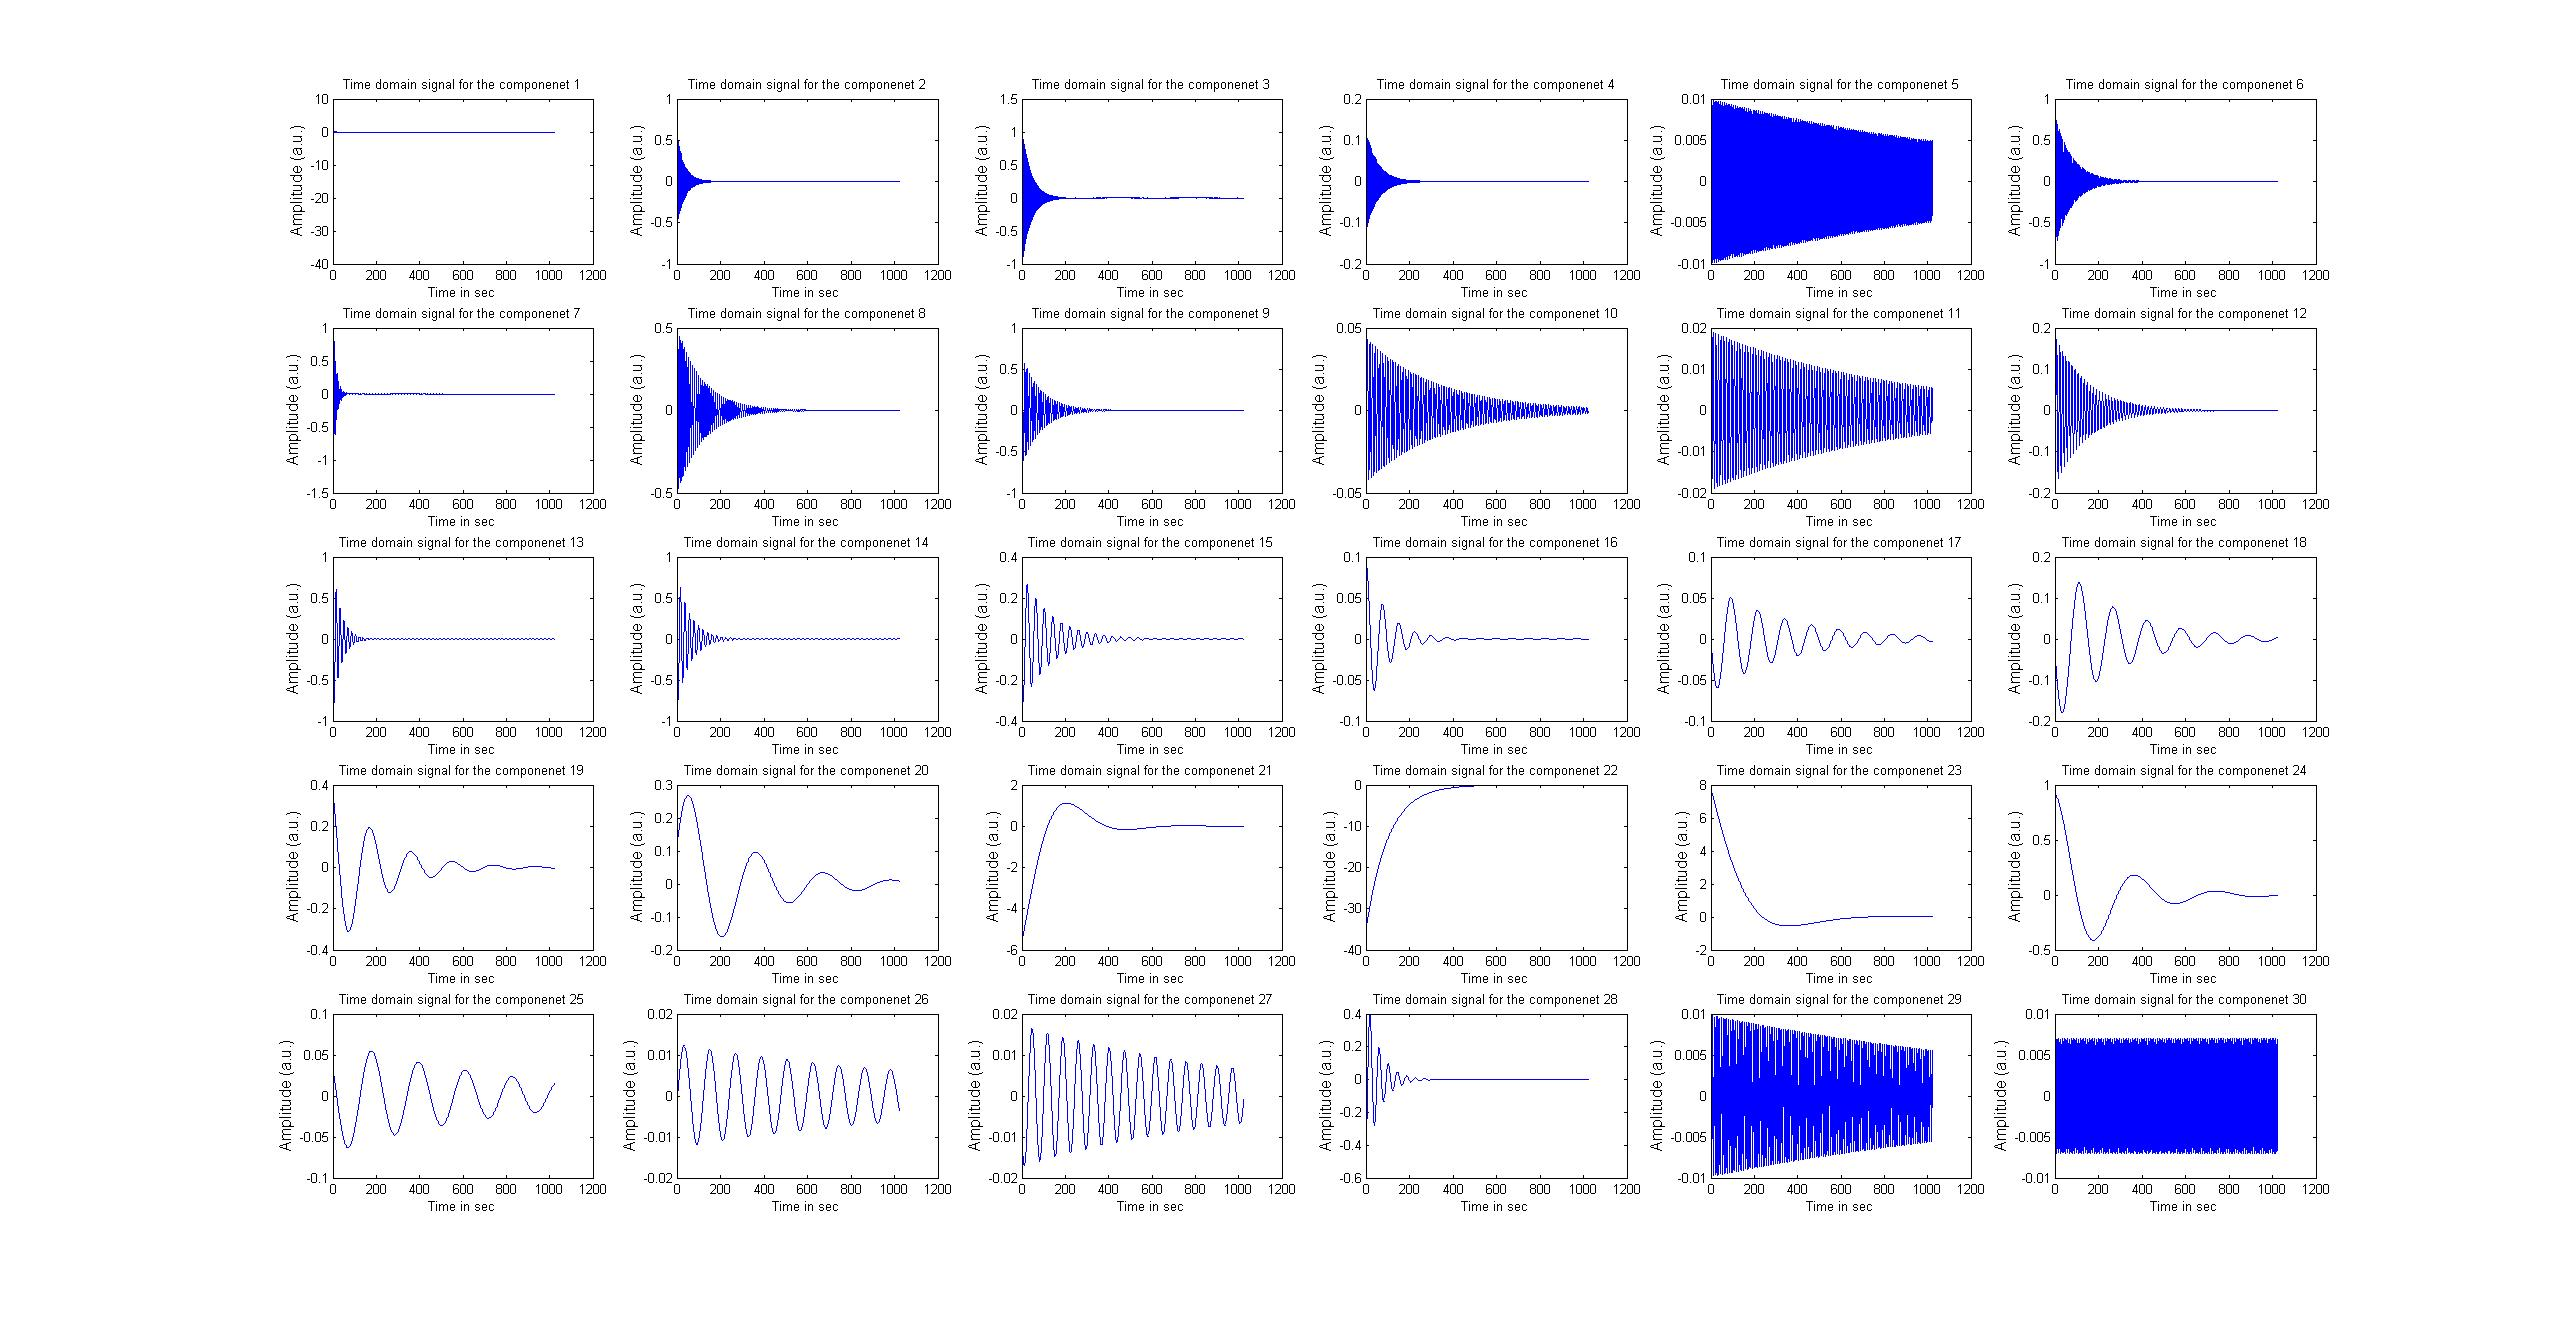
\includegraphics[width=1\textwidth]{6.jpg}
\subcaption{Time domain components}
\end{figure}

\begin{figure}[!htbp]
\centering
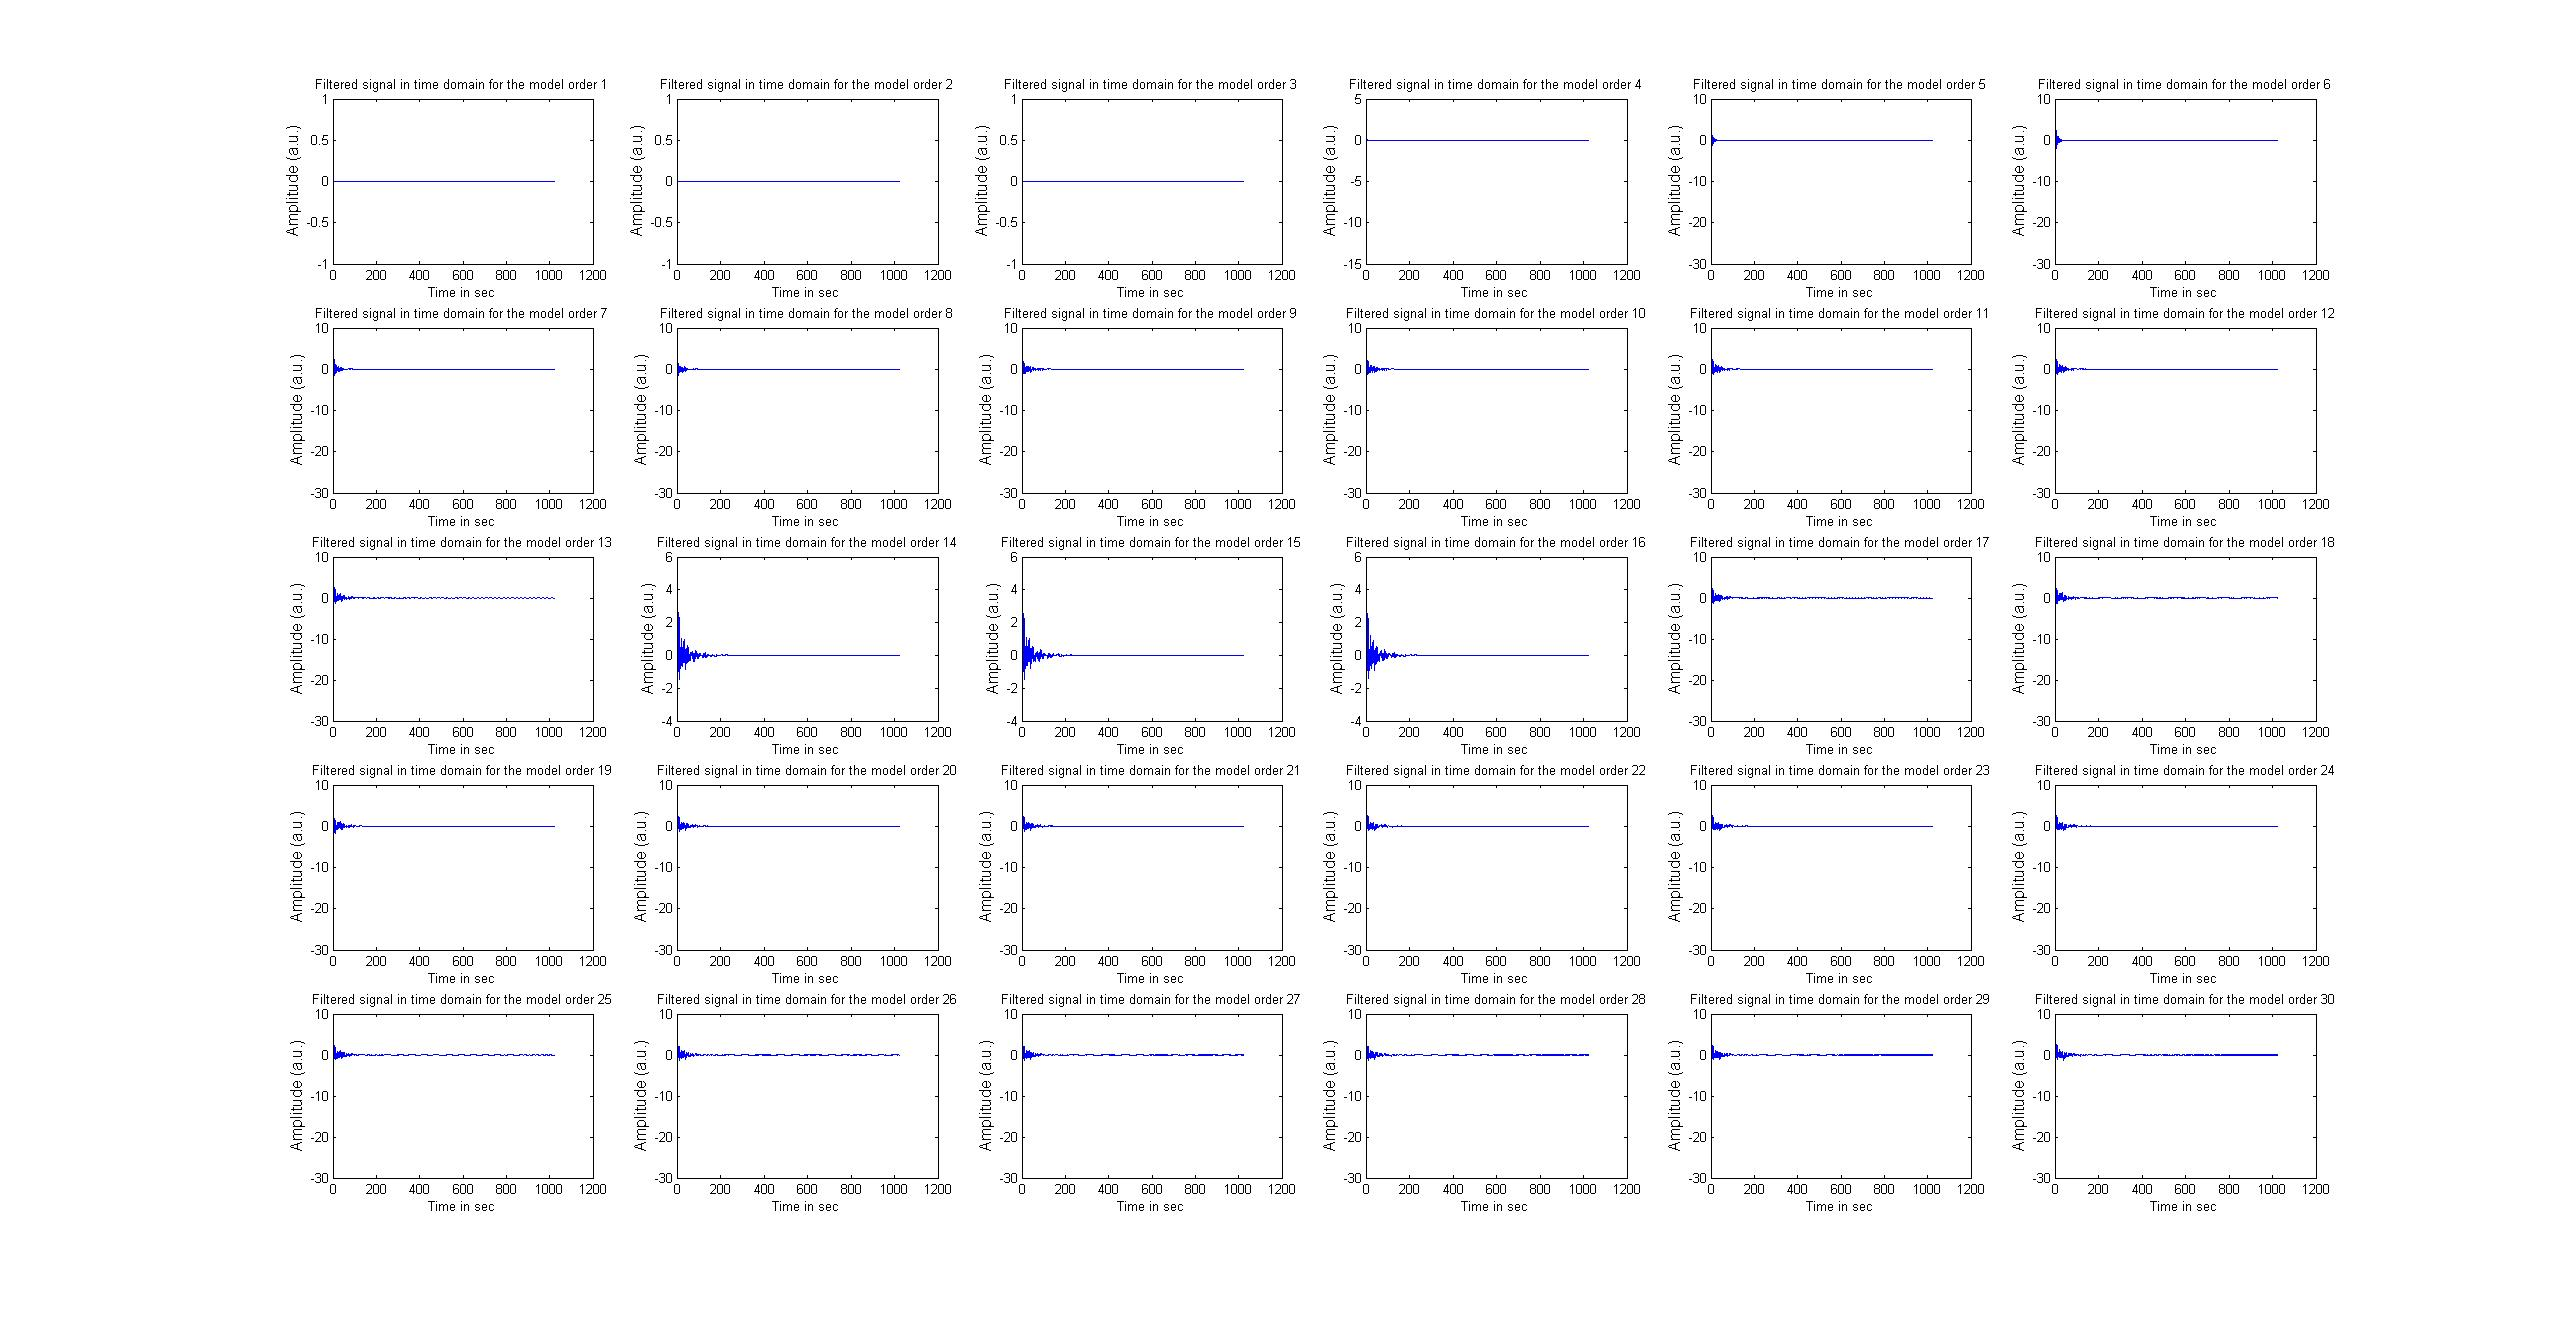
\includegraphics[width=1\textwidth]{7.jpg}
\caption{}
\end{figure}






\begin{figure}[!htbp]
\minipage{.5\textwidth}%
\centering
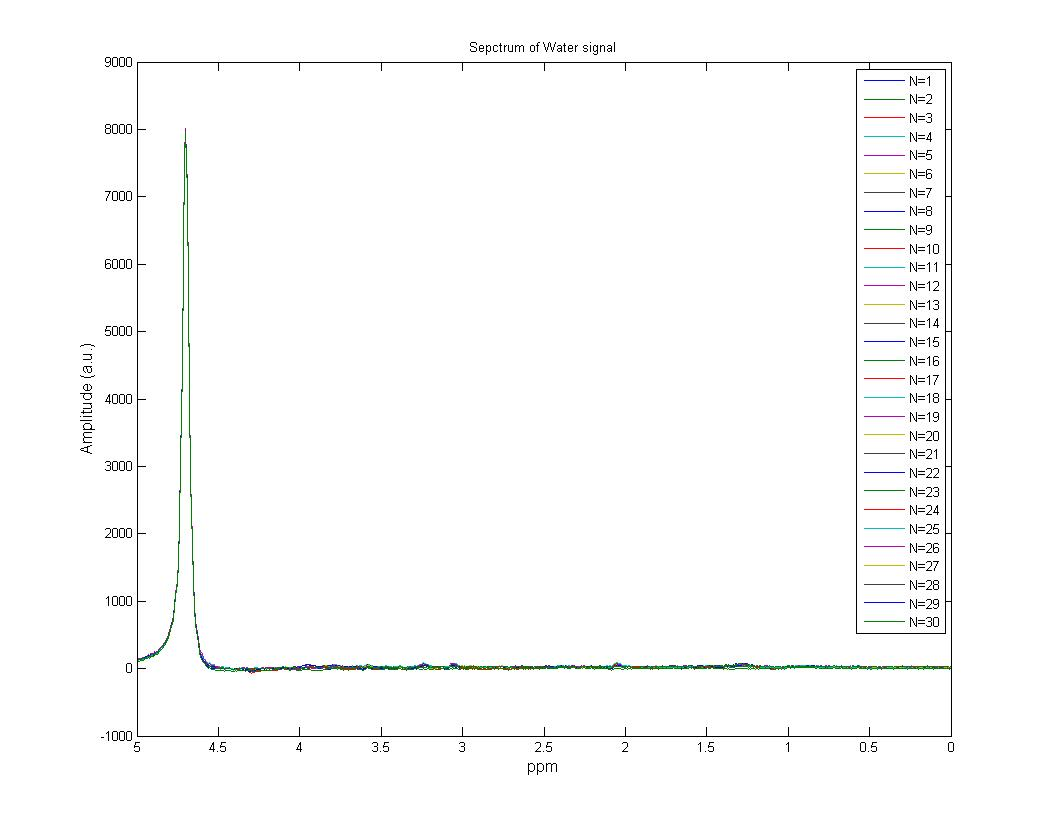
\includegraphics[width=1\textwidth]{9.jpg}
\subcaption{Spectrum water signal for different order model}\label{fig5}
\endminipage\hfill
\minipage{.5\textwidth}%
\centering
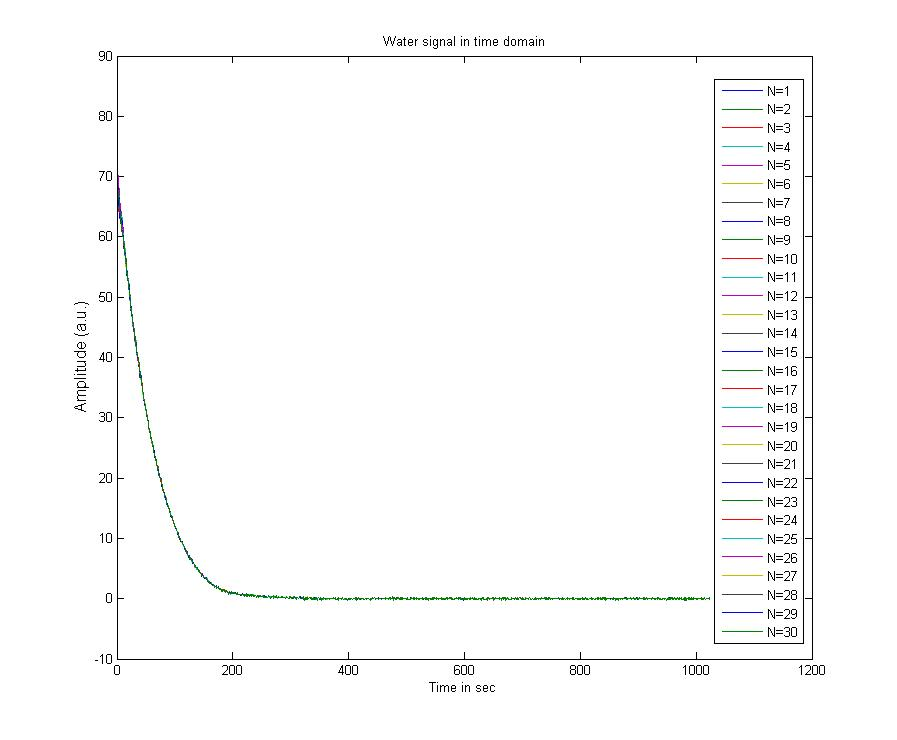
\includegraphics[width=1\textwidth]{10.jpg}
\subcaption{Water signal in time domain for different order model}\label{fig4}
\endminipage\hfill
\caption{}
\end{figure}

\begin{figure}[!htbp]
\centering
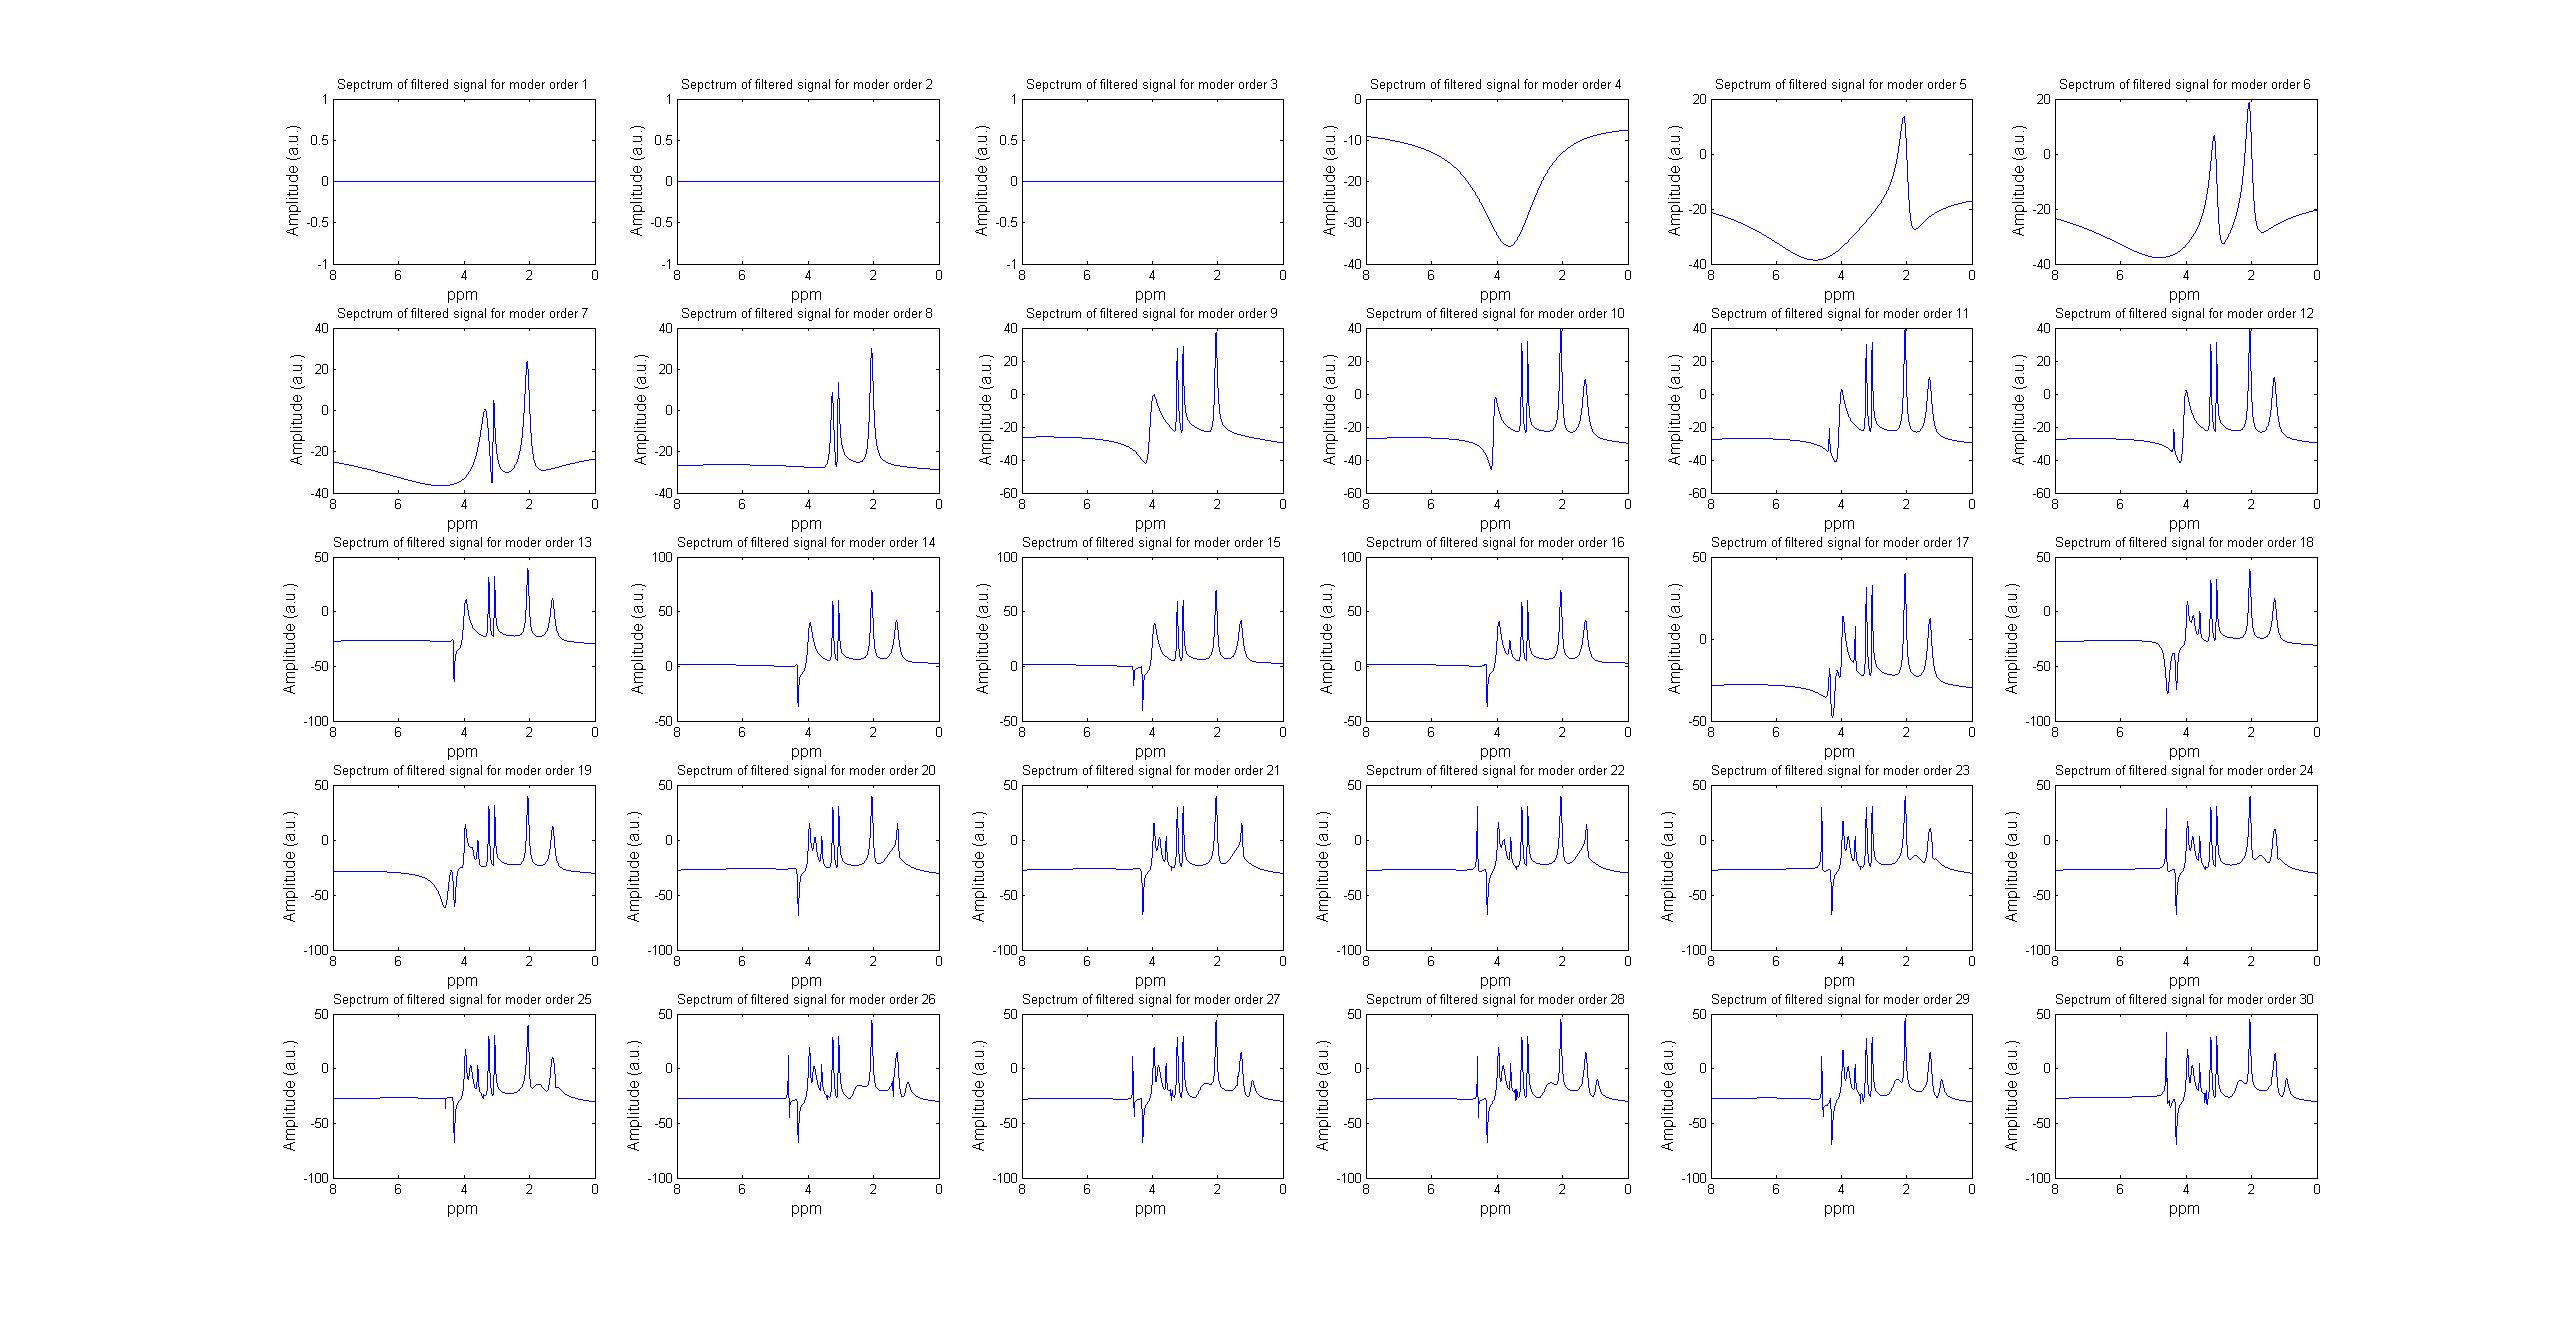
\includegraphics[width=1\textwidth]{8_2.jpg}
\caption{Spectrum Water filtered signal for different order model}\label{fig6}
\end{figure}

\begin{figure}[!htbp]
\centering
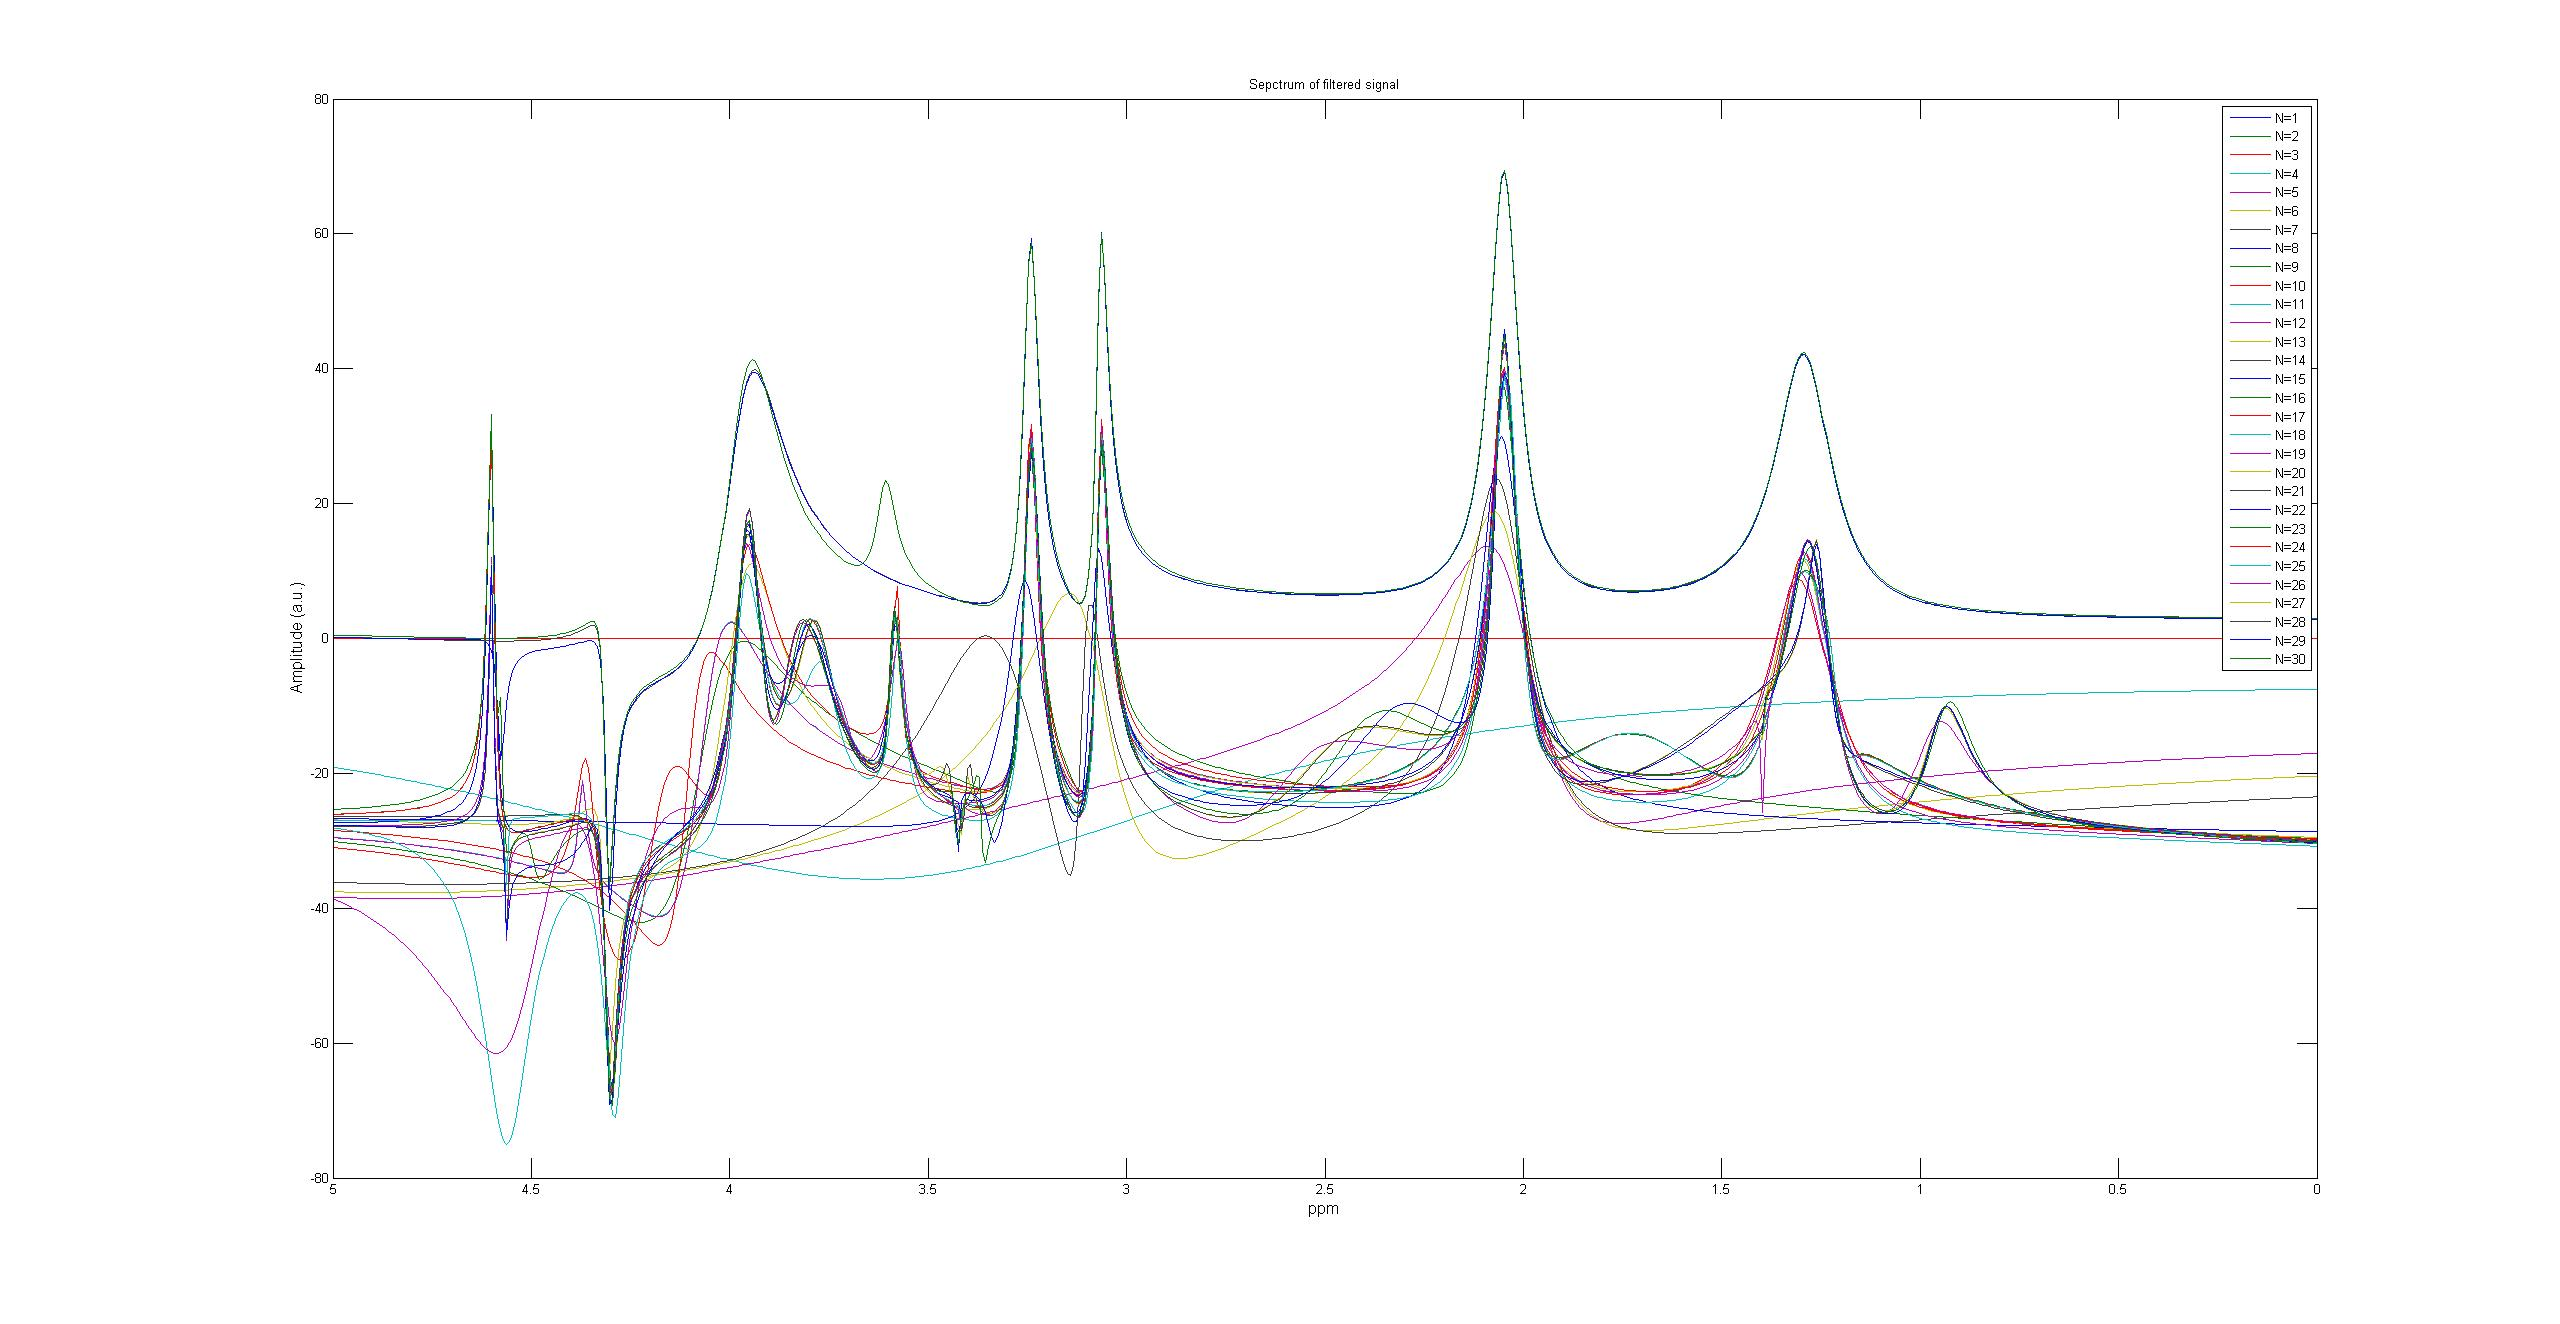
\includegraphics[width=1\textwidth]{8.jpg}
\caption{Spectrum Water filtered signal for different order model}\label{fig7}
\end{figure}




\begin{equation}\label{eq1}
y(t)=\sum_{k=1}^{K} a_{k}exp(j\phi_{k})exp(-d_{k}t+2\pi f_{k}t)\delta t
\end{equation}

\begin{equation}
ppm=\frac{f_{Hz}*10^6}{f_{s}}-ppm_{Ref}
\end{equation}
\section{Additional figure}


\begin{figure}[!htbp]
\centering
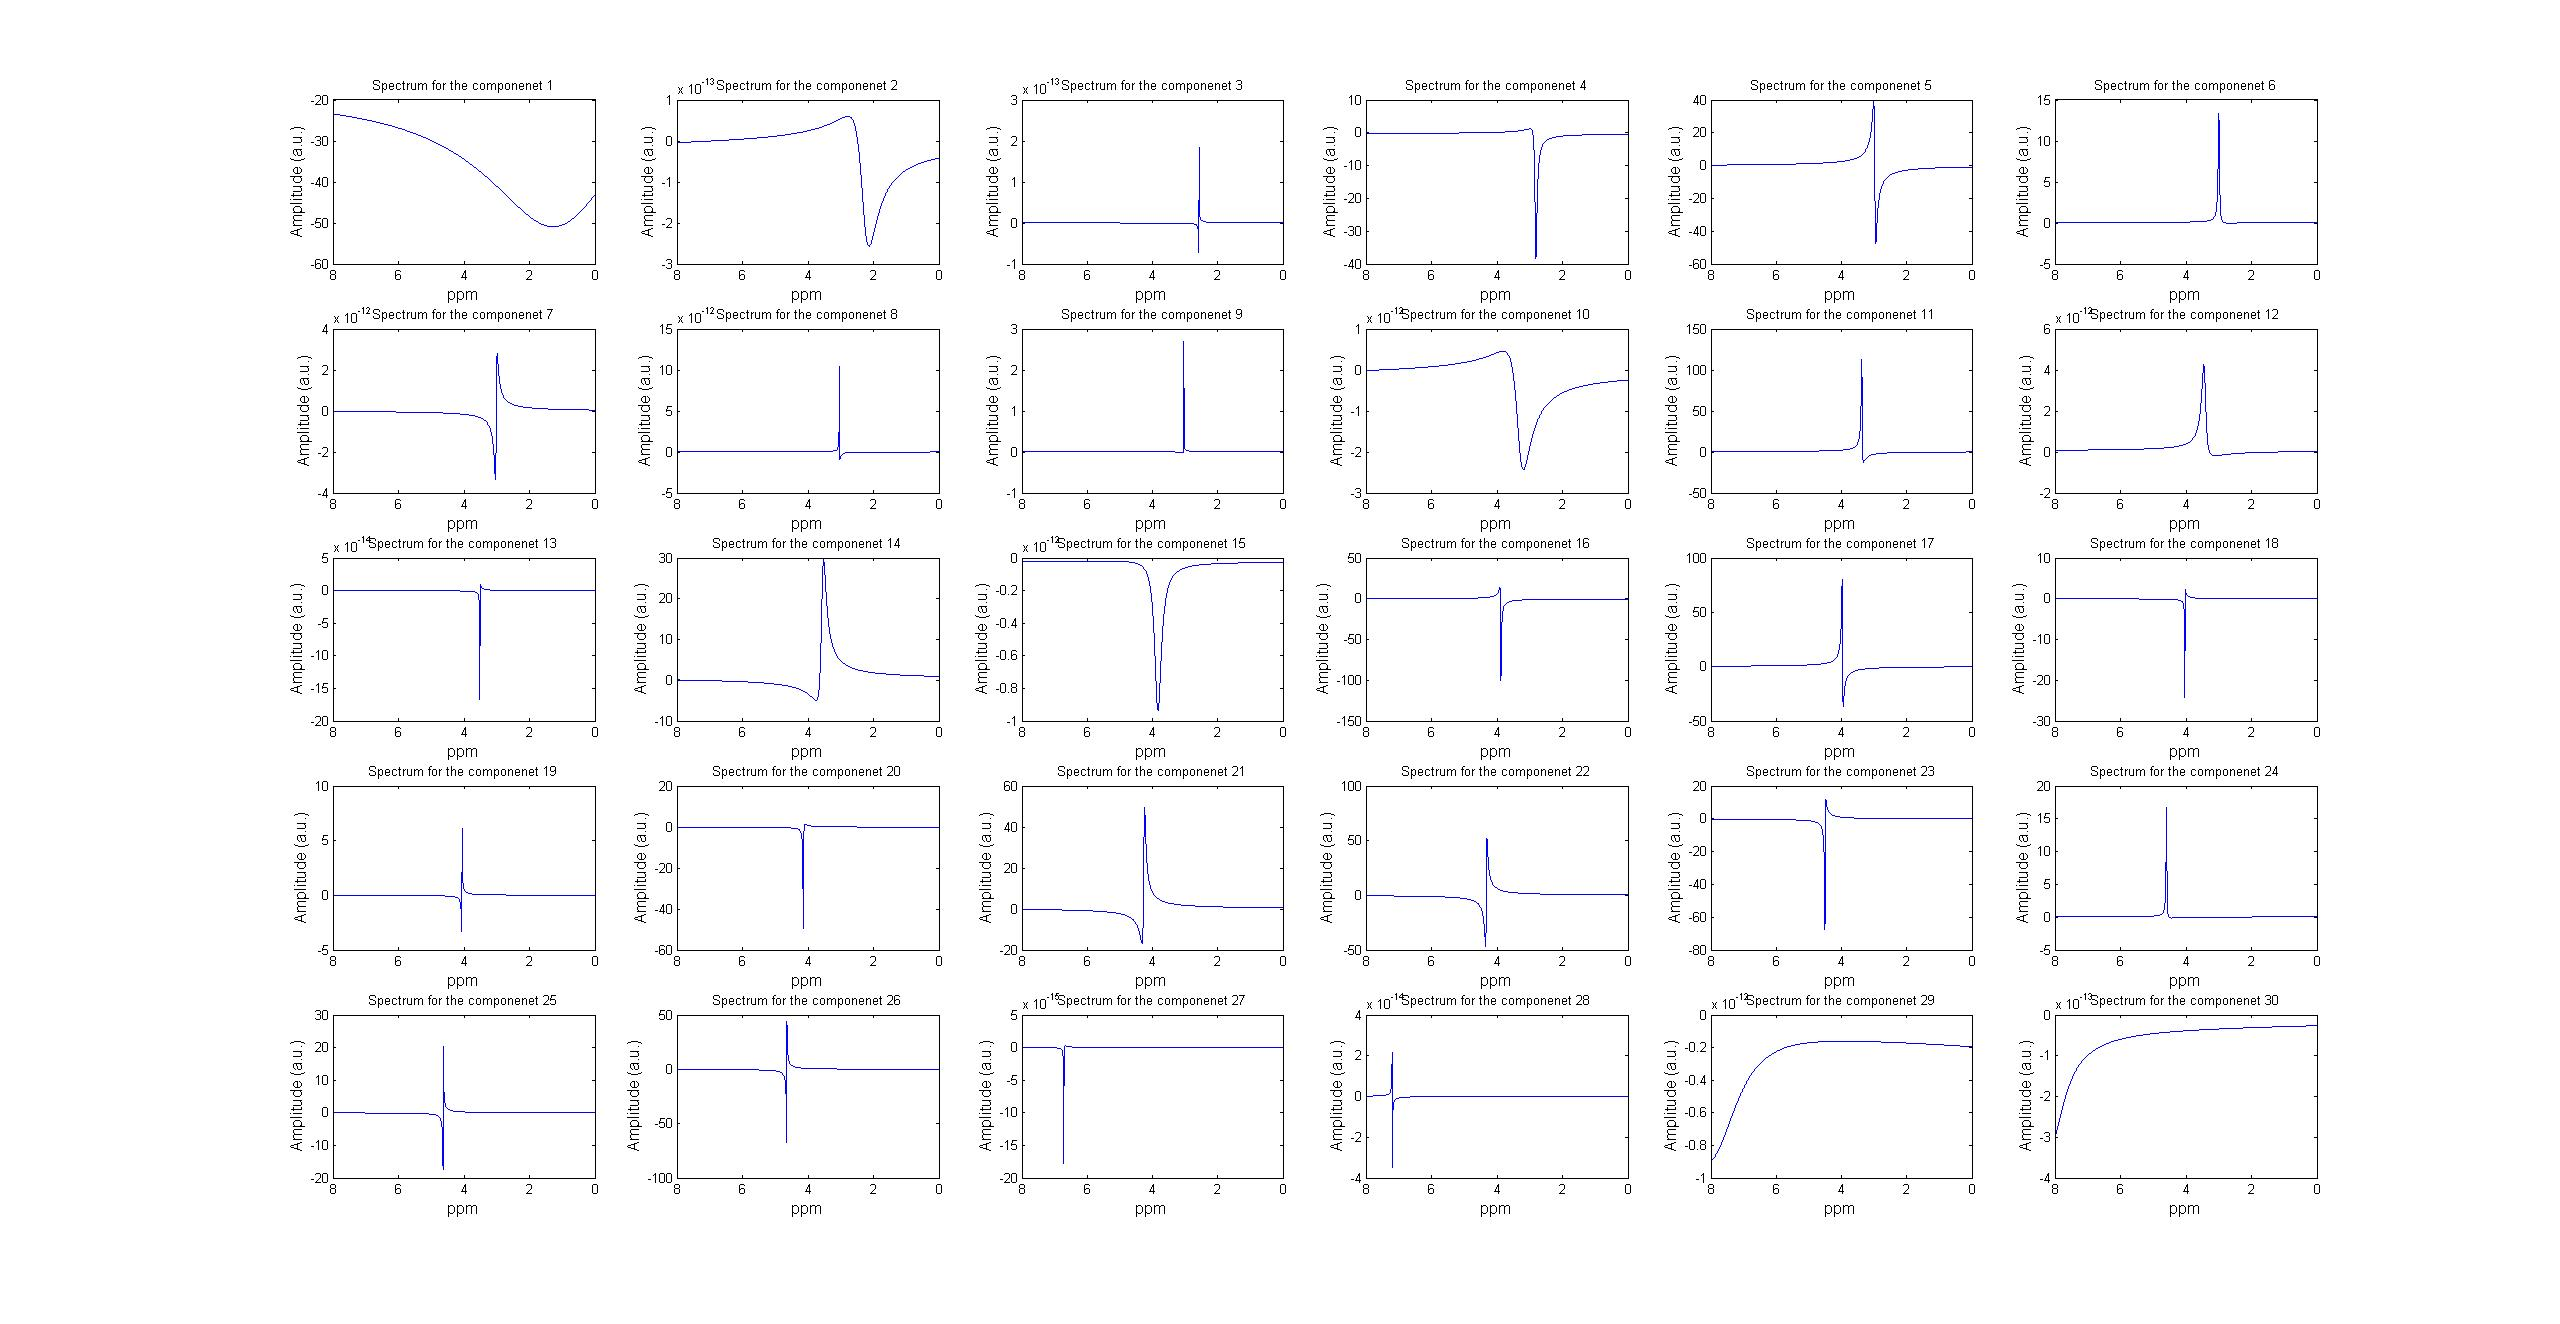
\includegraphics[width=1\textwidth]{16.jpg}
\caption{Individual component of the hsvd of the water filtered signal}
\end{figure}

\begin{figure}[!htbp]
\centering
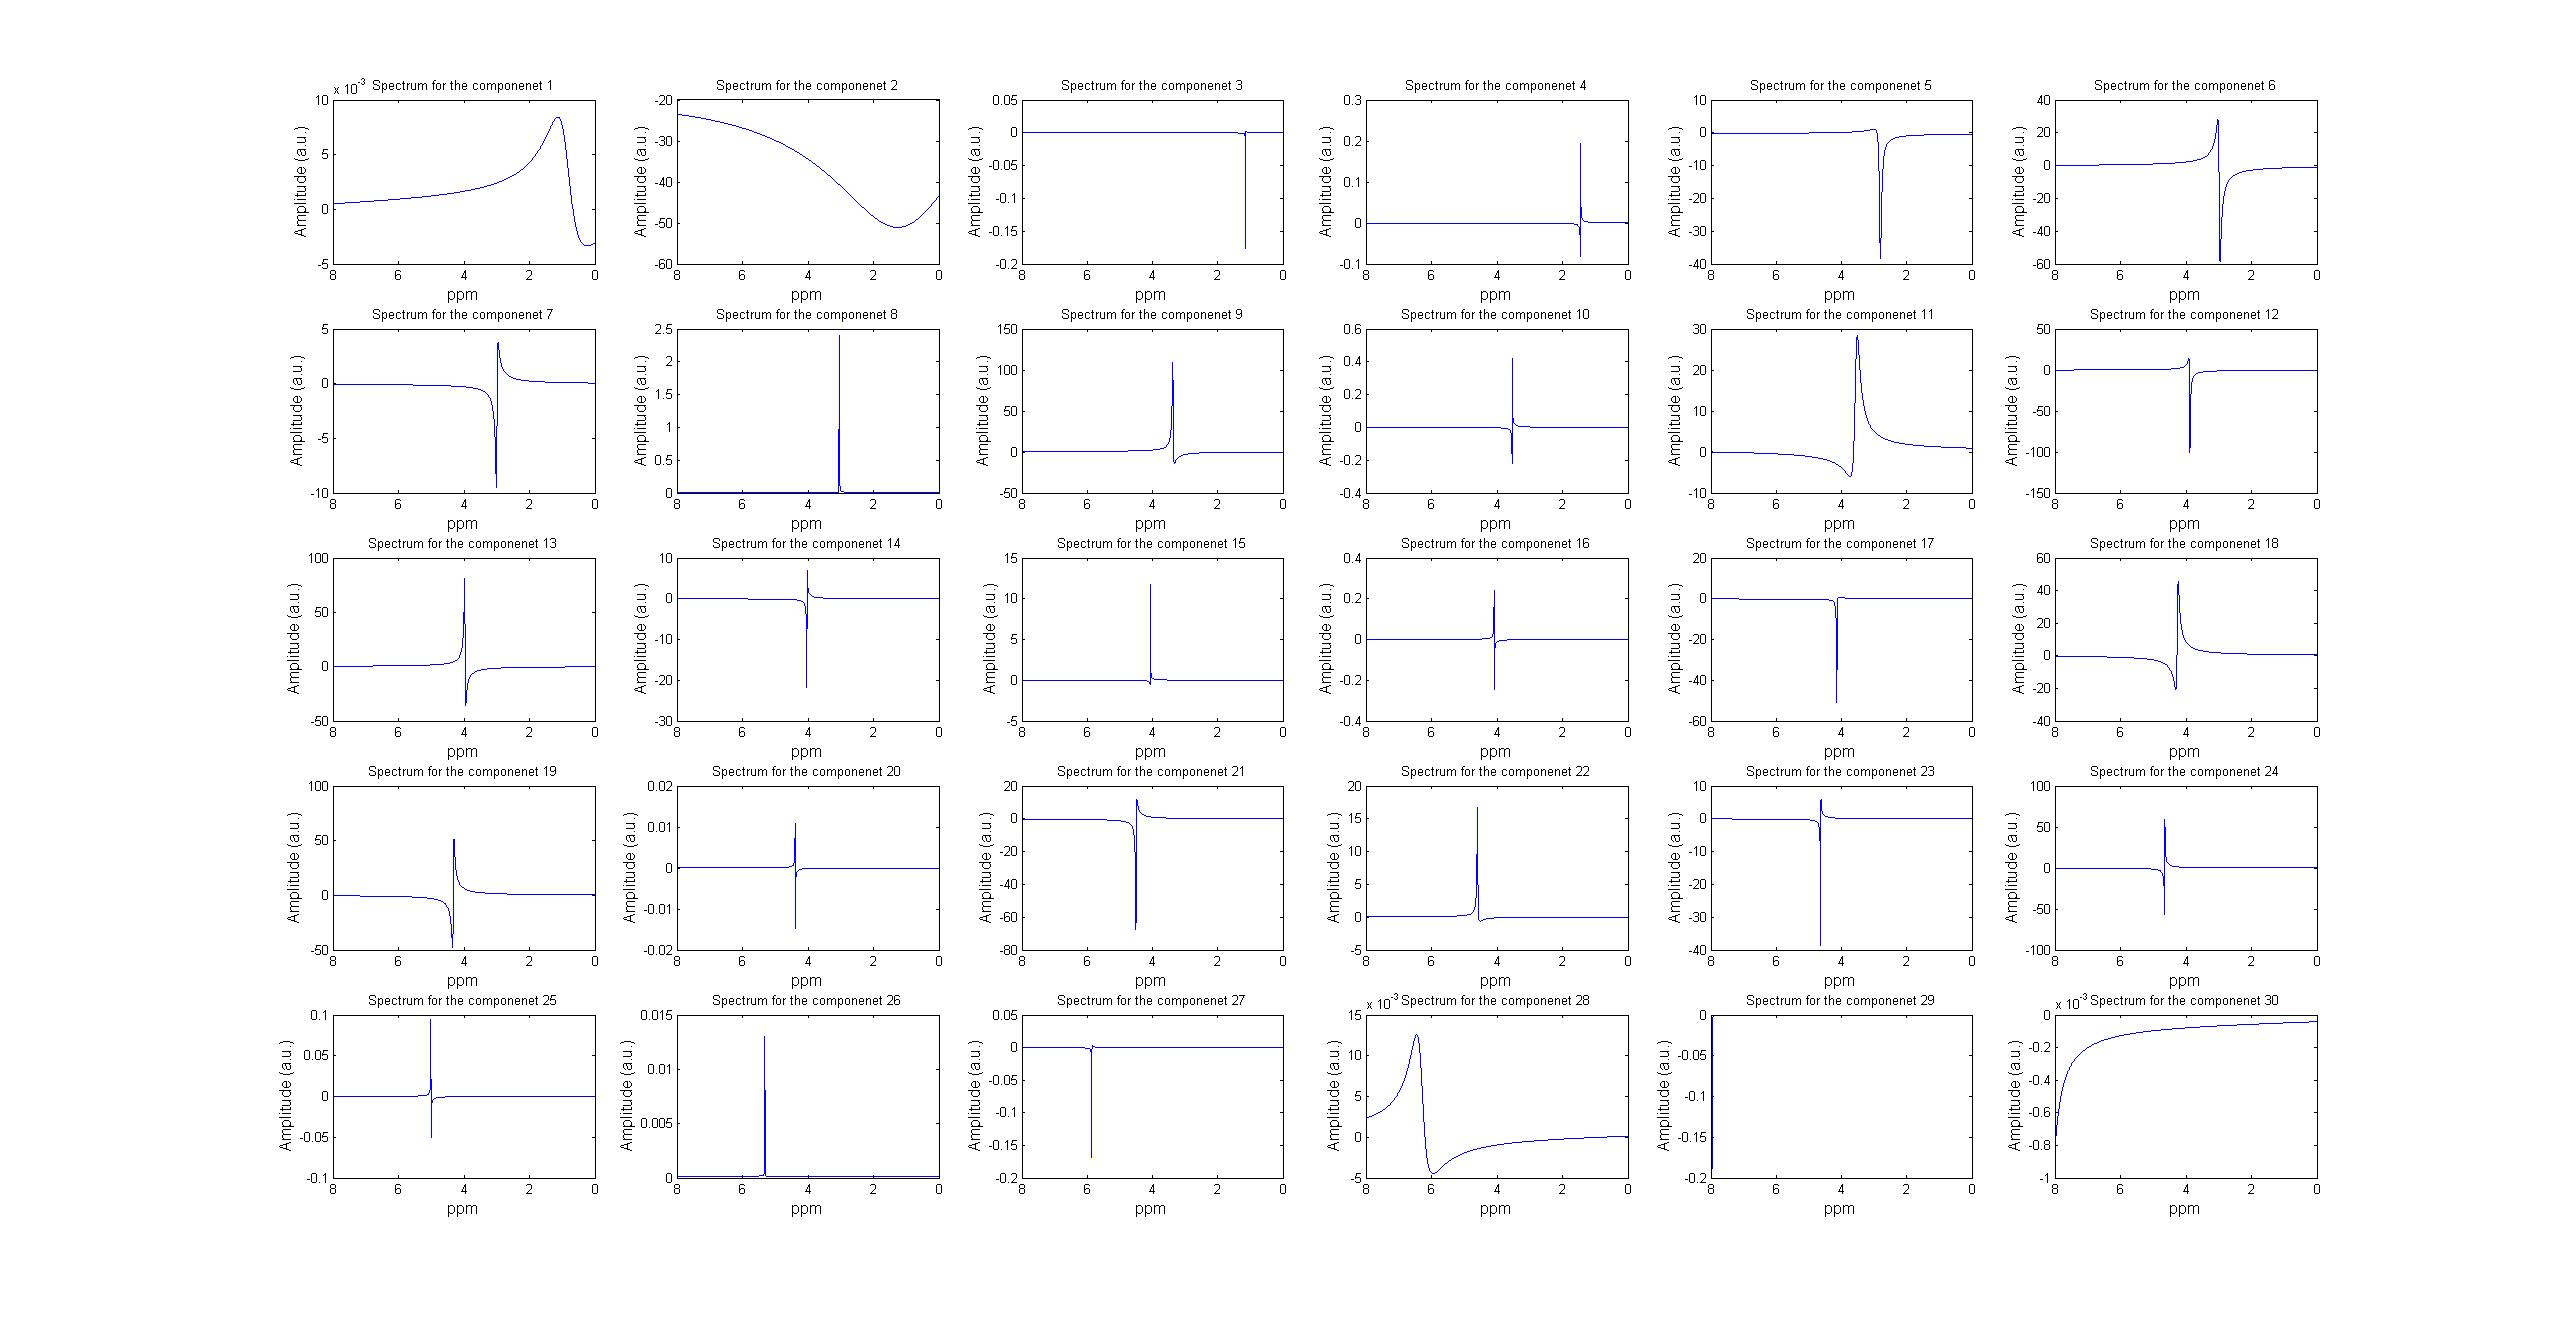
\includegraphics[width=1\textwidth]{17.jpg}
\caption{Individual component of the hsvd of the noisy water filtered signal}
\end{figure}

\begin{figure}[!htbp]
\centering
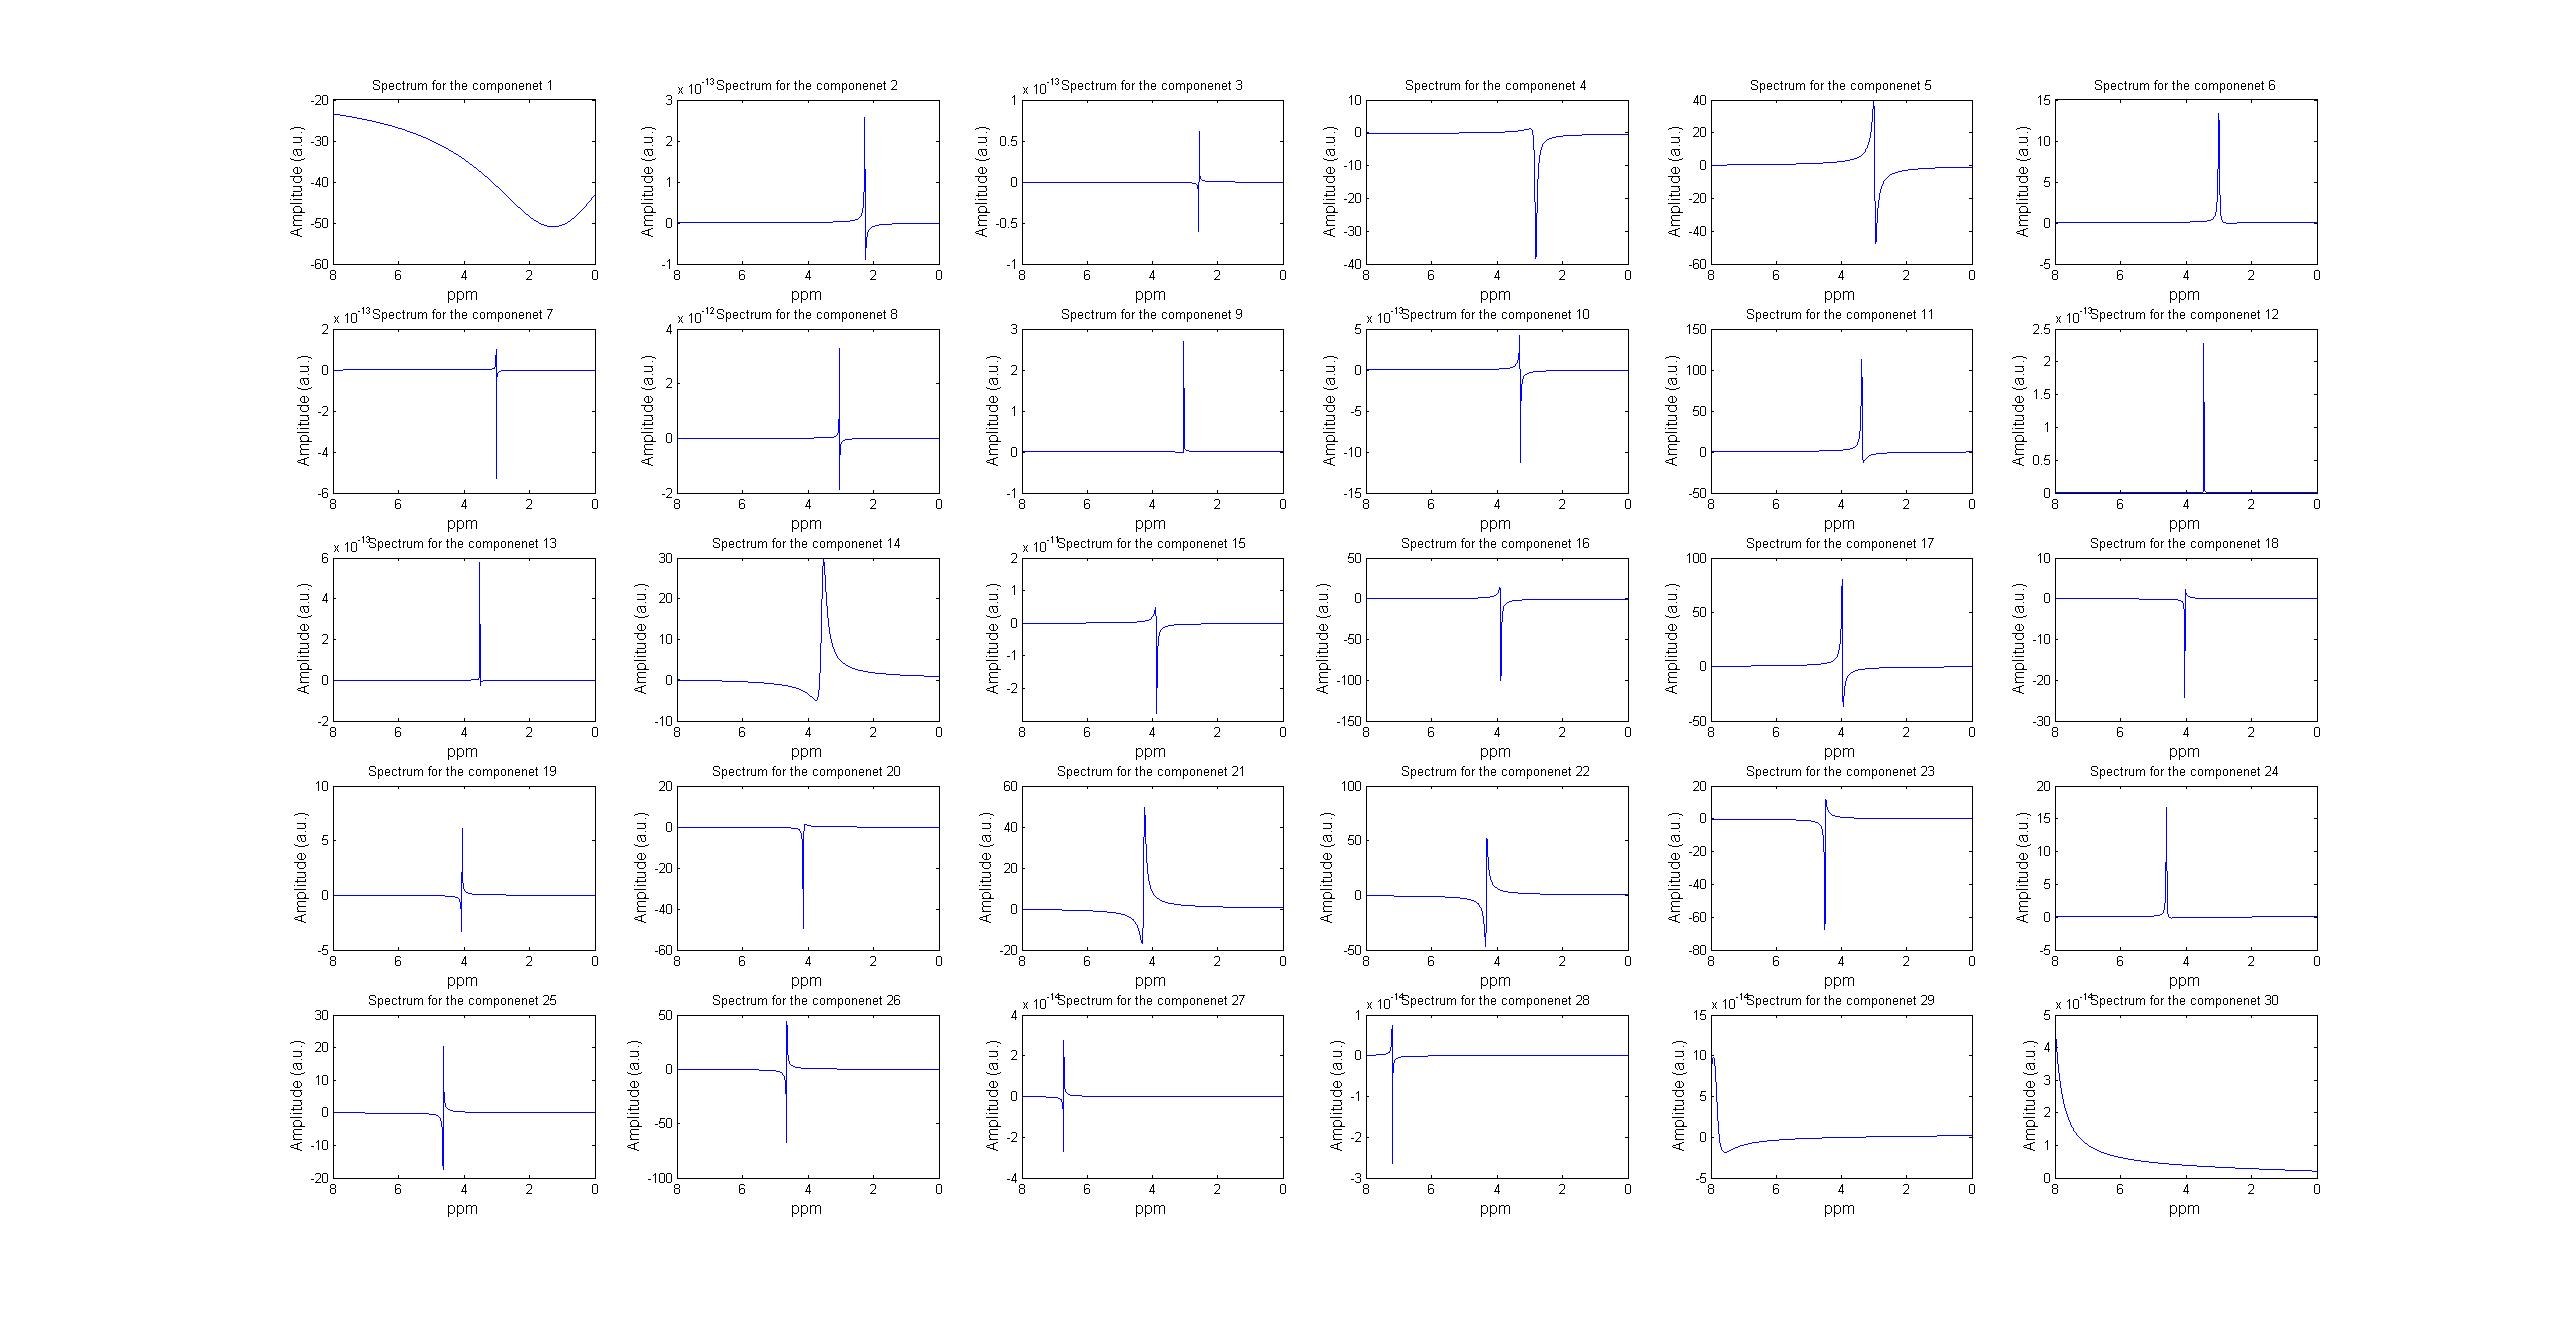
\includegraphics[width=1\textwidth]{18.jpg}
\caption{Individual component of the htlsU of the water filtered signal}
\end{figure}

\begin{figure}[!htbp]
\centering
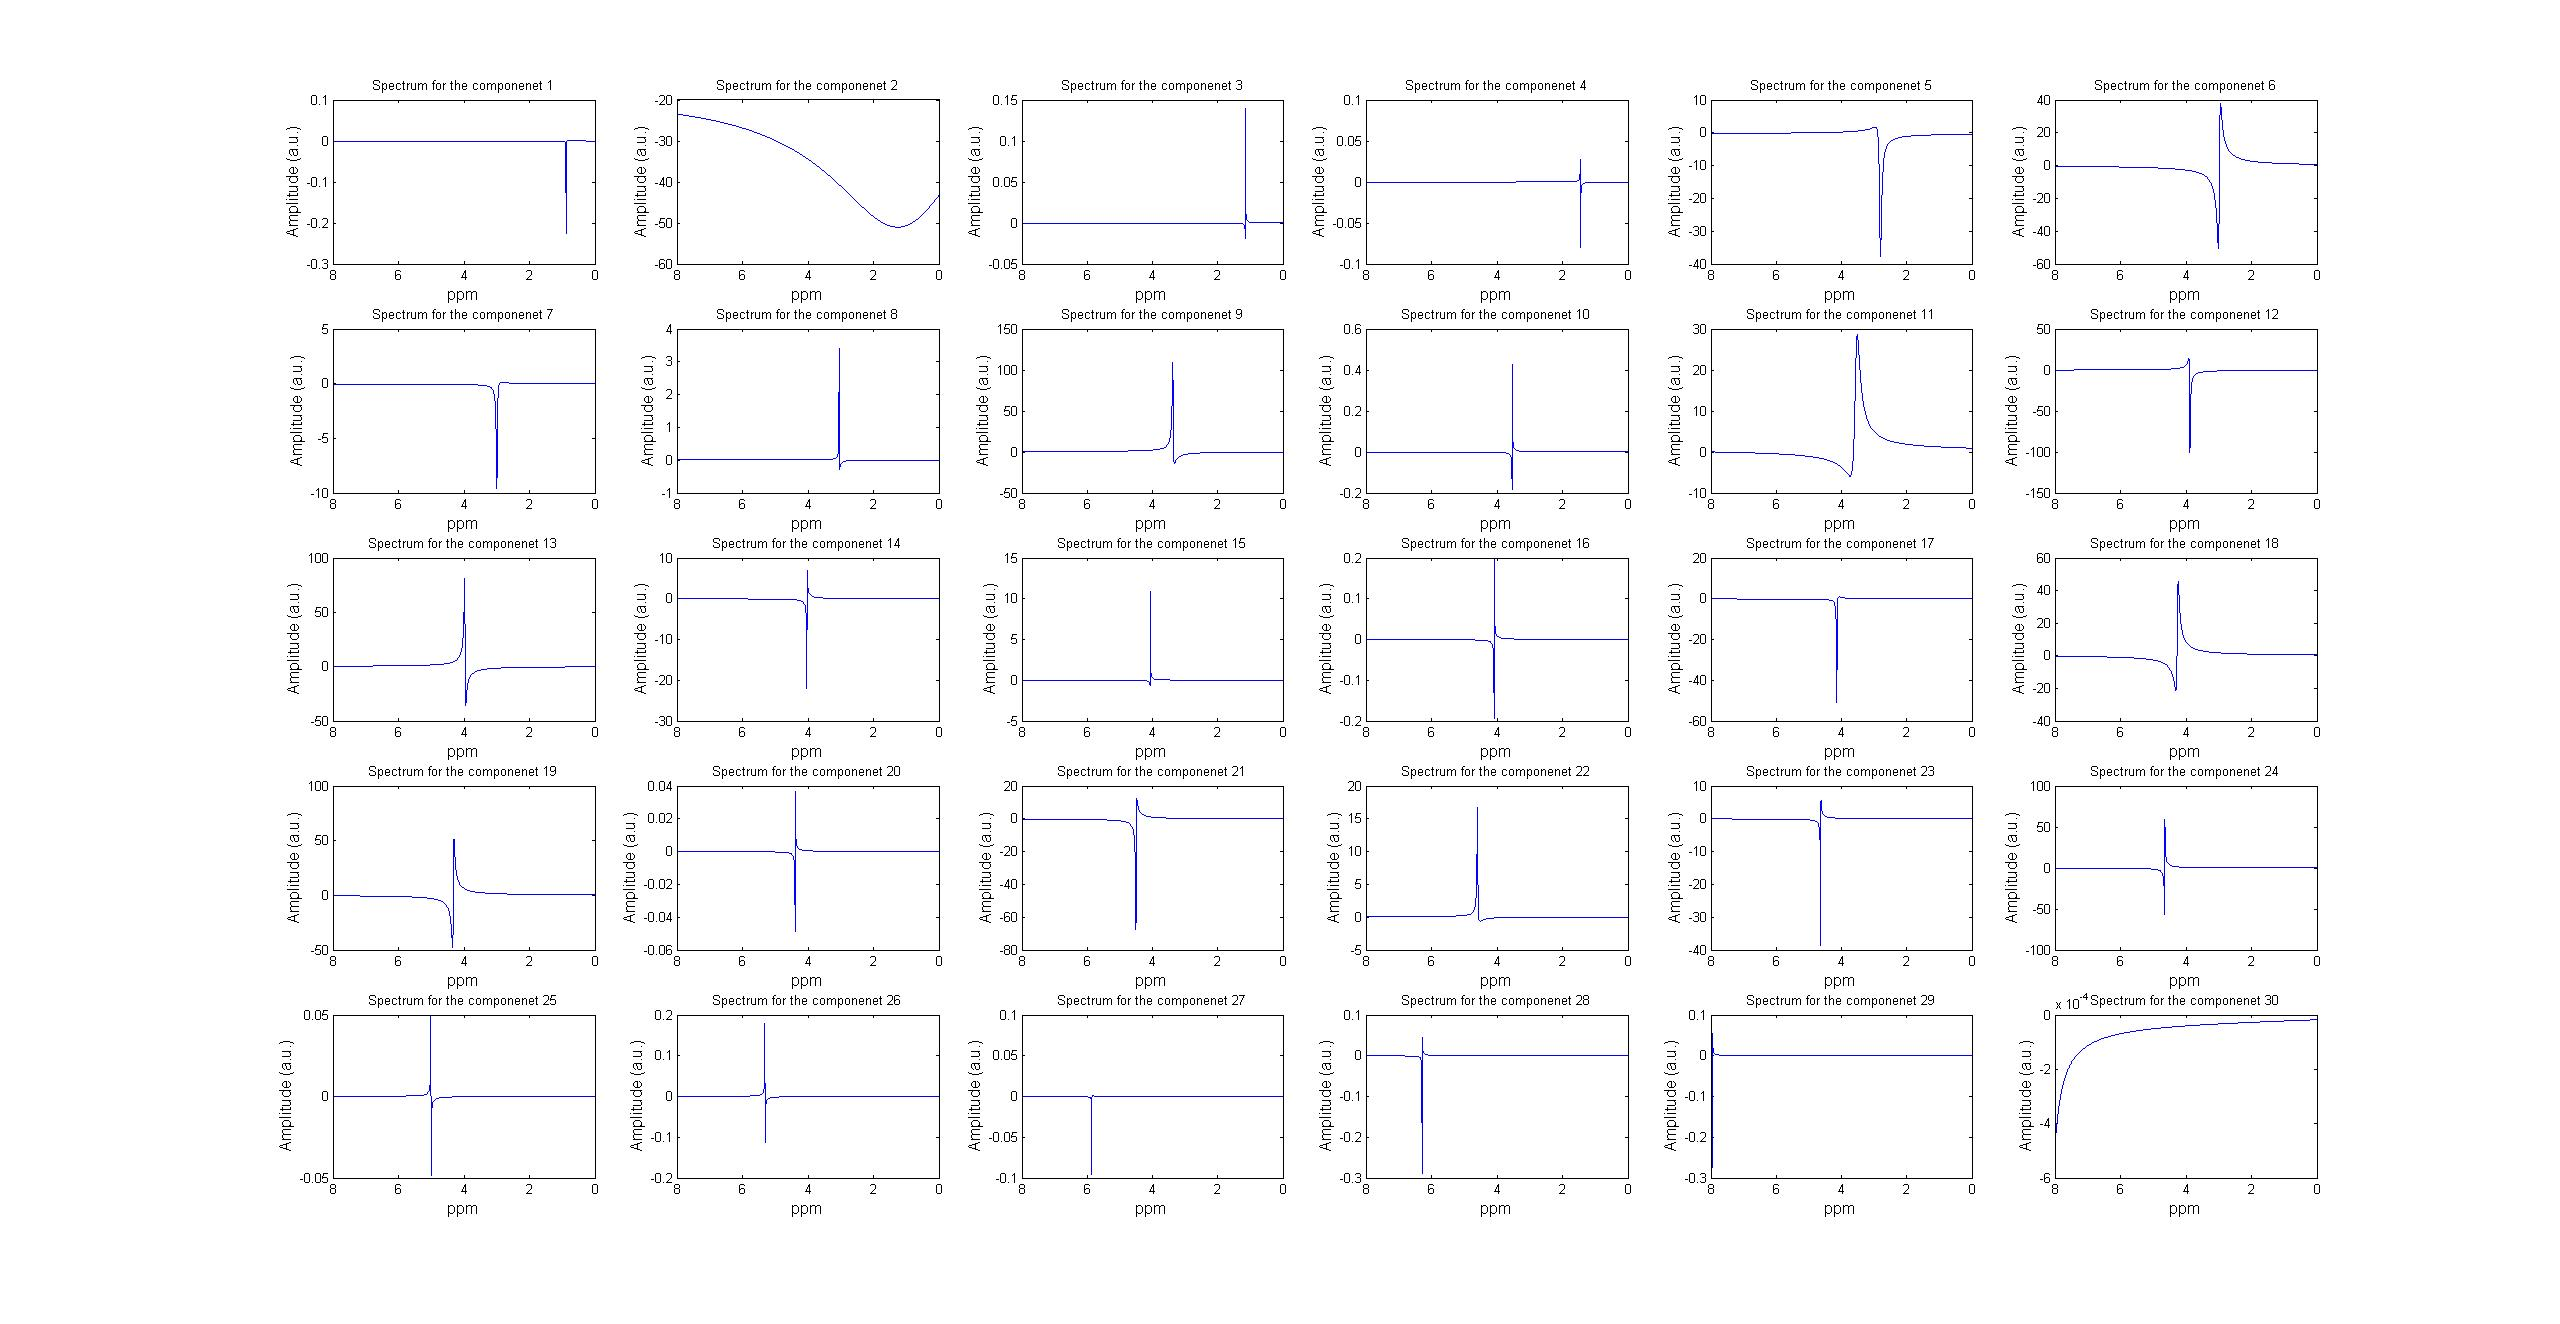
\includegraphics[width=1\textwidth]{19.jpg}
\caption{Individual component of the htlsU of the noisy water filtered signal}
\end{figure}

\begin{figure}[!htbp]
\centering
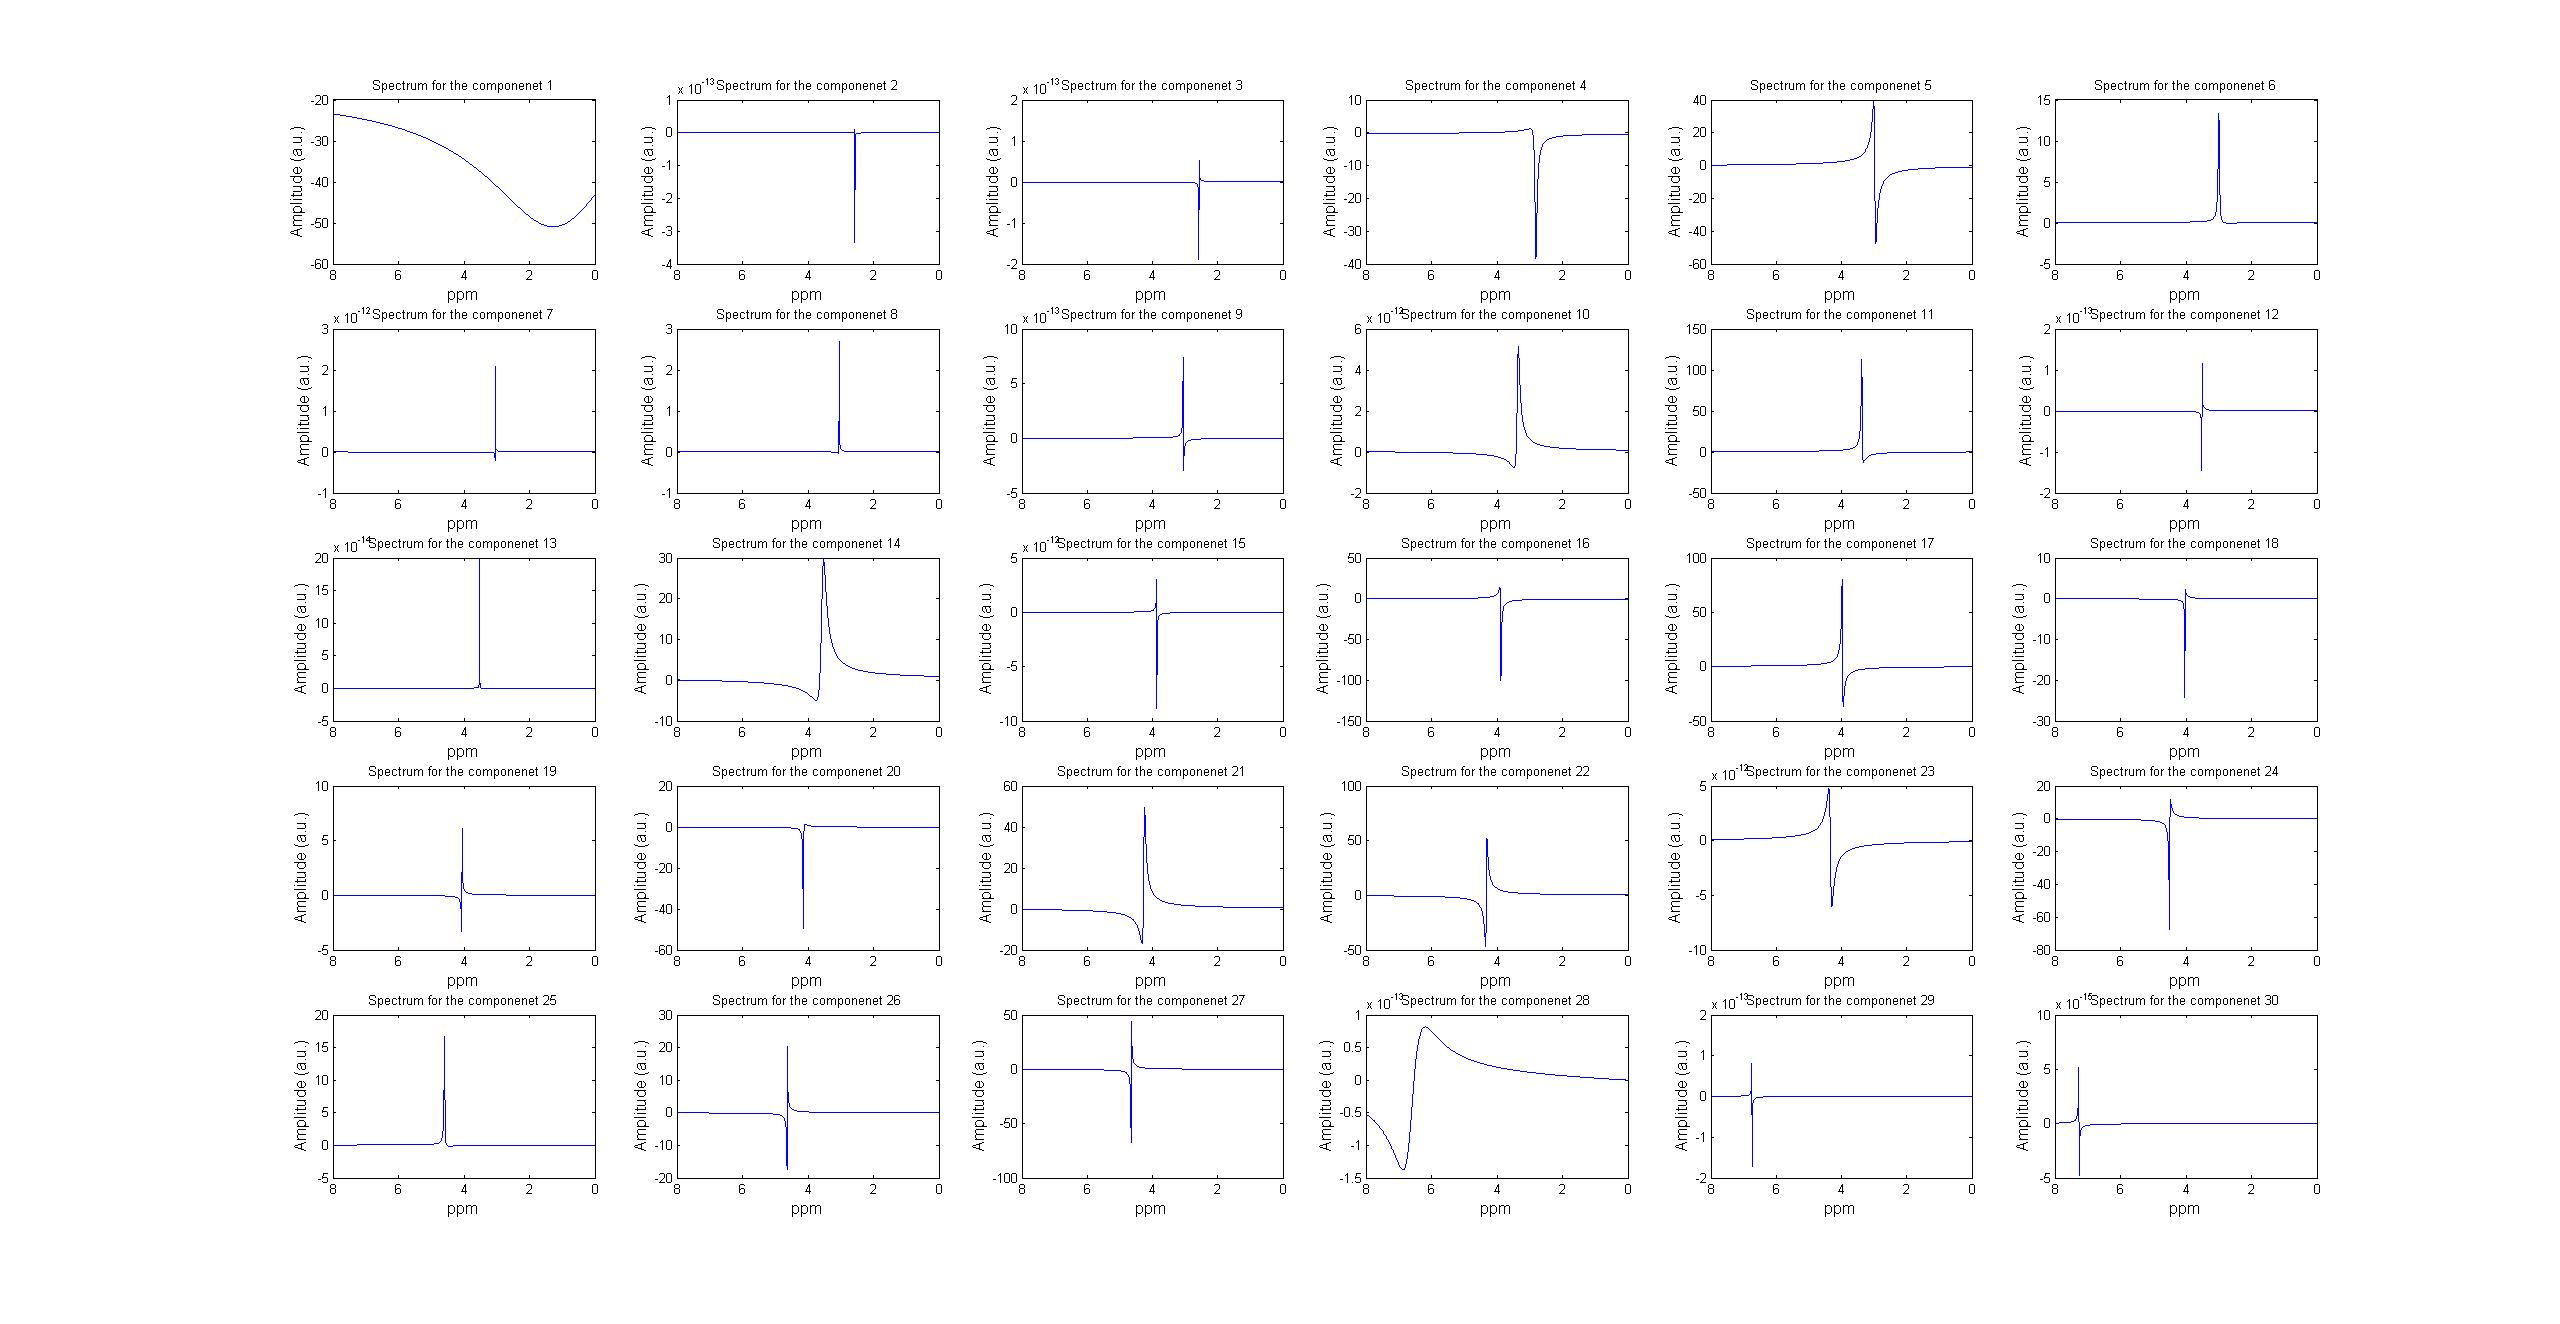
\includegraphics[width=1\textwidth]{20.jpg}
\caption{Individual component of the htlspkfd of the water filtered signal}
\end{figure}

\begin{figure}[!htbp]
\centering
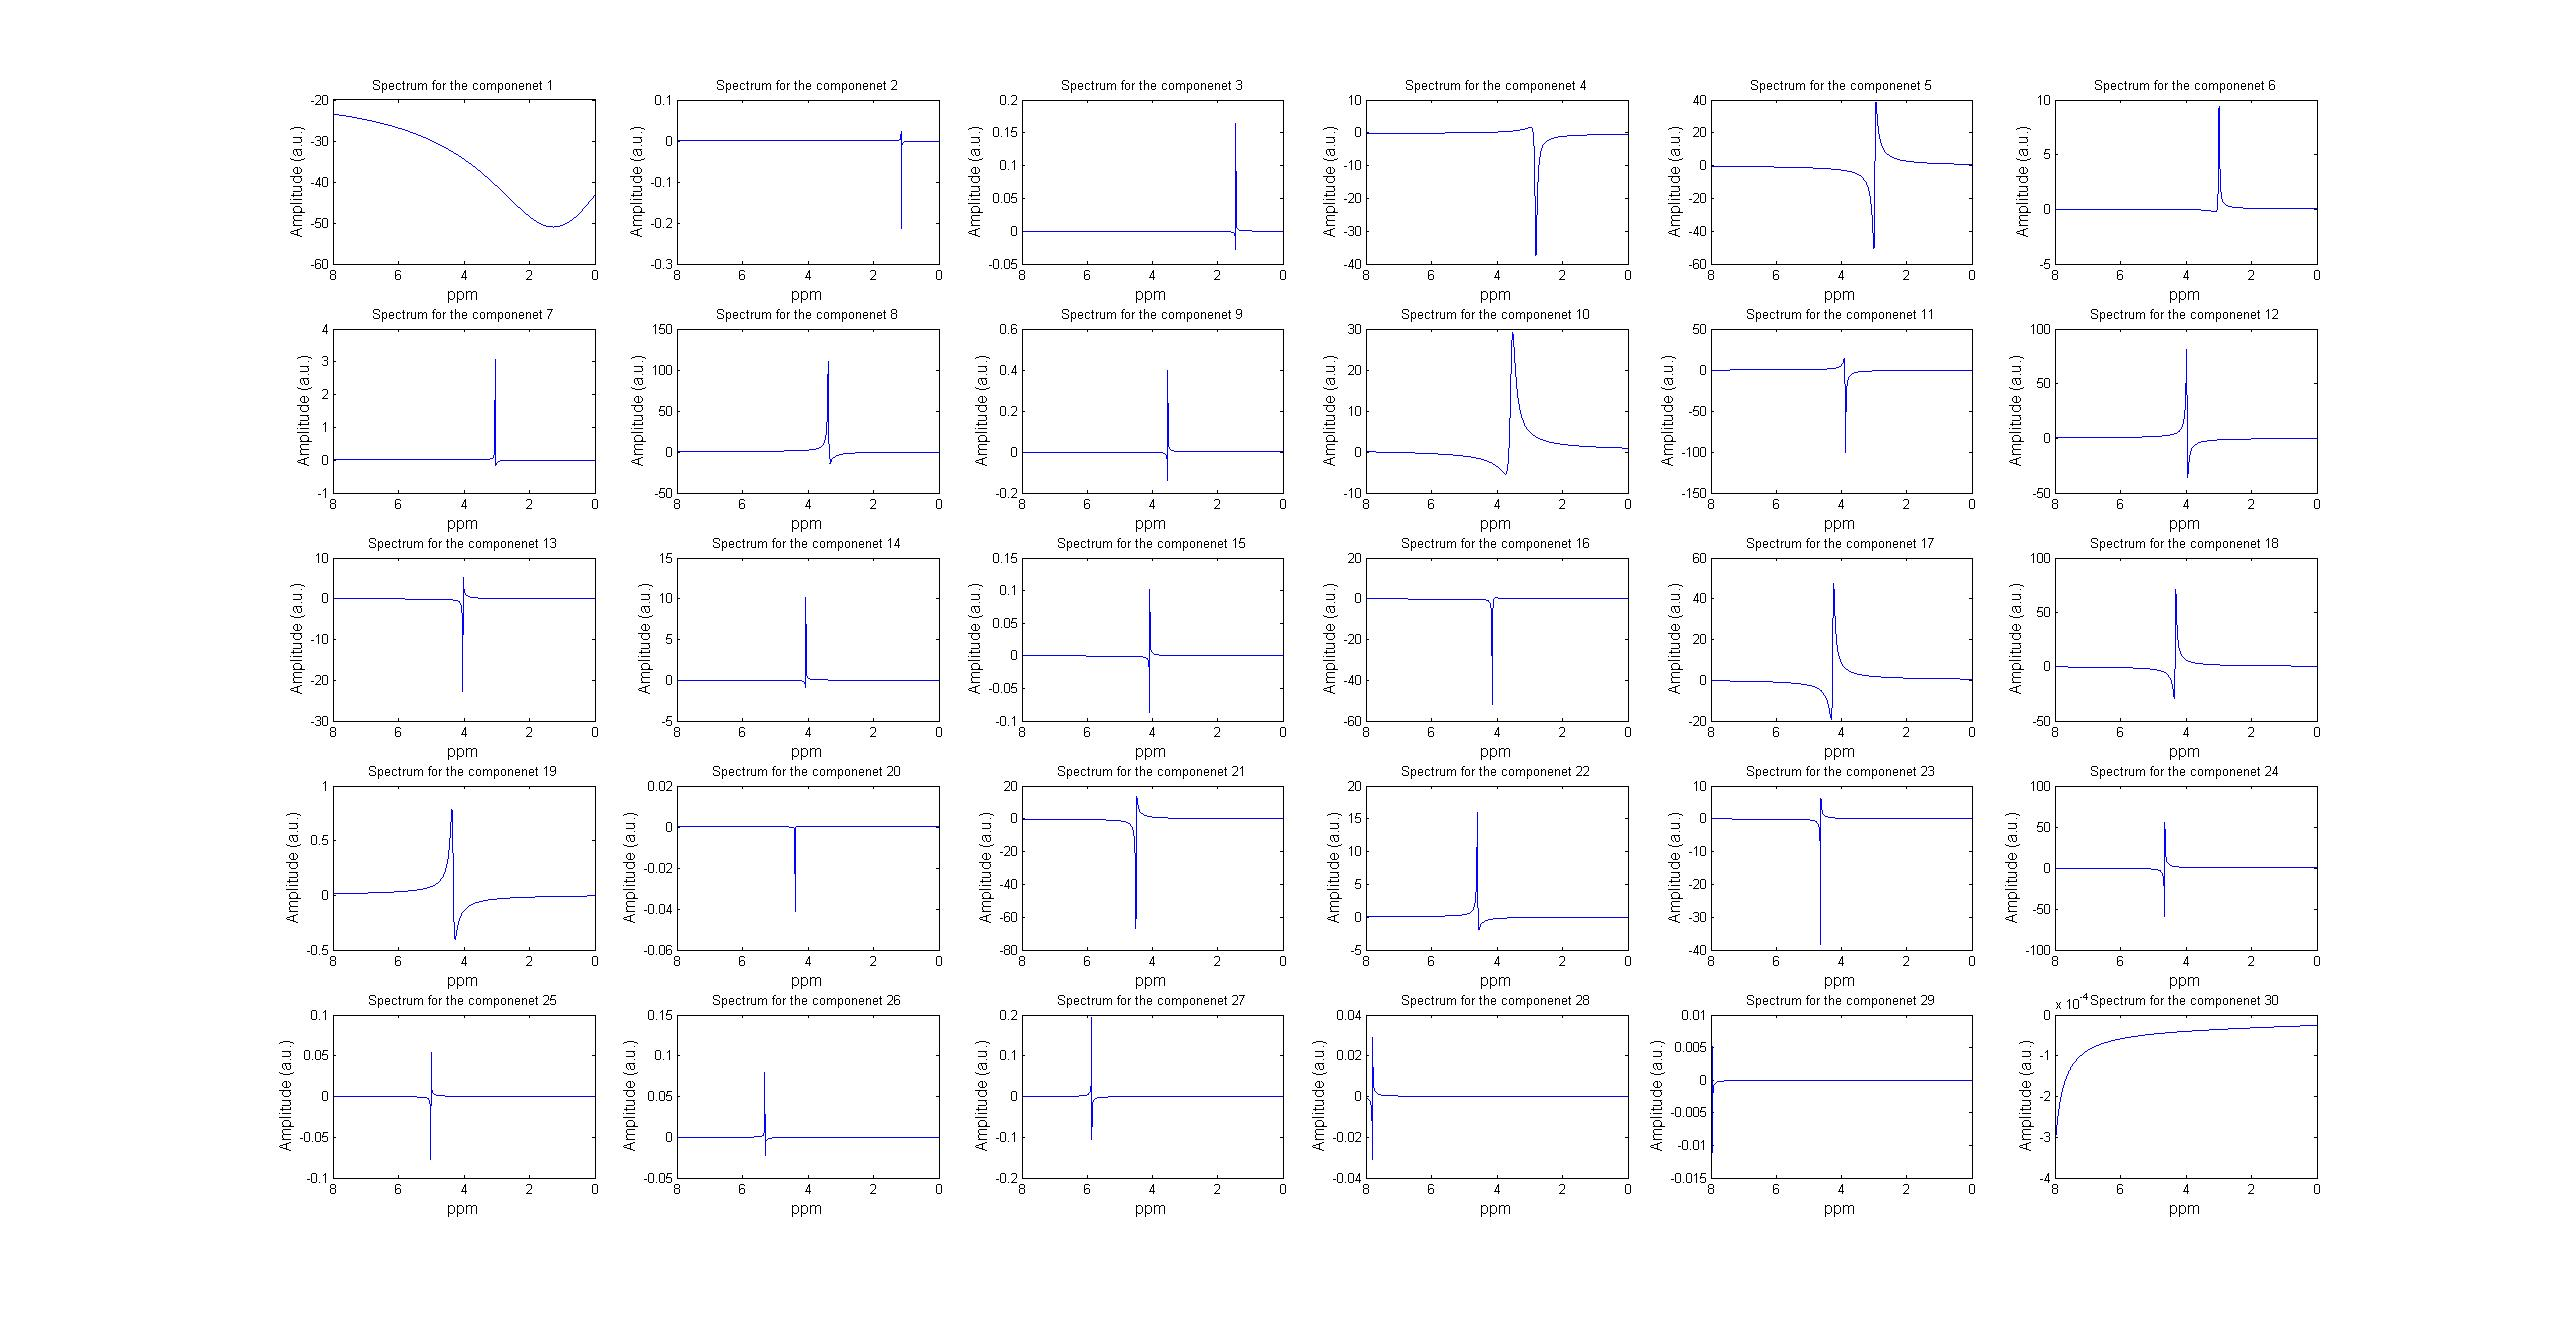
\includegraphics[width=1\textwidth]{21.jpg}
\caption{Individual component of the htlspkfd of the noisy water filtered signal}
\end{figure}



\begin{figure}[!htbp]
\minipage{.5\textwidth}%
\centering
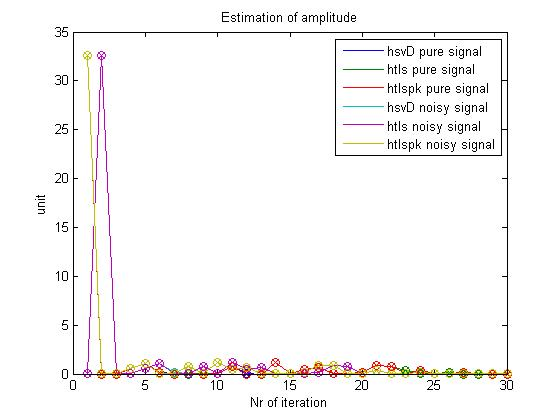
\includegraphics[width=1\textwidth]{12.jpg}
\subcaption{}
\endminipage\hfill
\minipage{.5\textwidth}%
\centering
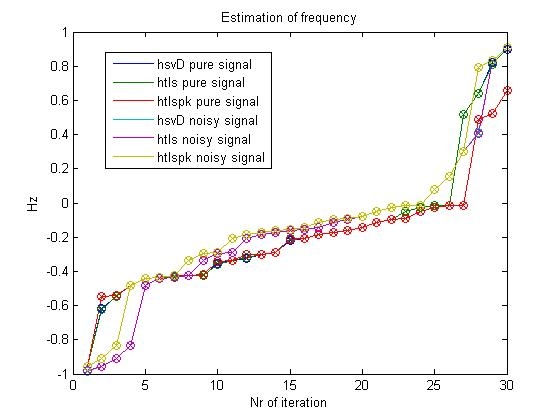
\includegraphics[width=1\textwidth]{13.jpg}
\subcaption{}
\endminipage\hfill
\minipage{.5\textwidth}%
\centering
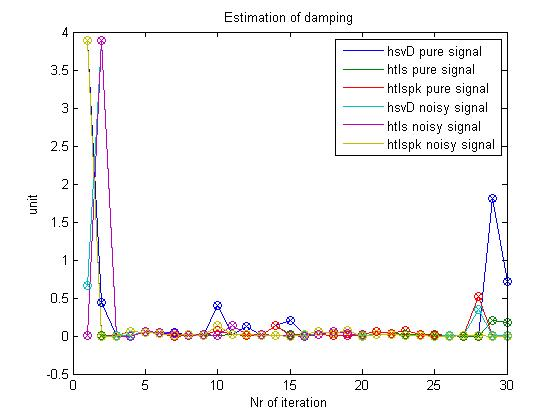
\includegraphics[width=1\textwidth]{14.jpg}
\subcaption{}
\endminipage\hfill
\minipage{.5\textwidth}%
\centering
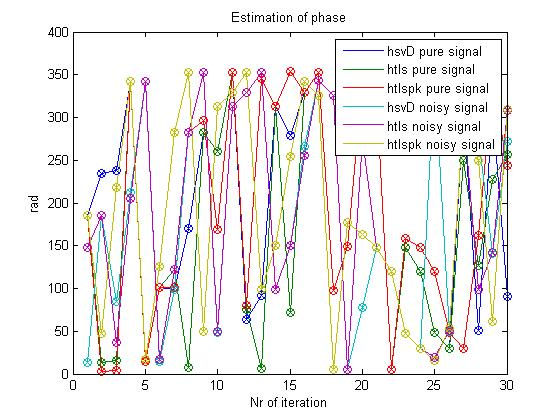
\includegraphics[width=1\textwidth]{15.jpg}
\subcaption{}
\endminipage\hfill
\caption{}
\end{figure}







\section{Additional figure}

\begin{figure}[!htbp]
\centering

\includegraphics[width=1\textwidth]{37.jpg}
\caption{A 9x9 voxel neighbourhood with the voxel of interest in the middle}\label{figtoda1}
\end{figure}

\begin{figure}[!htbp]
\centering
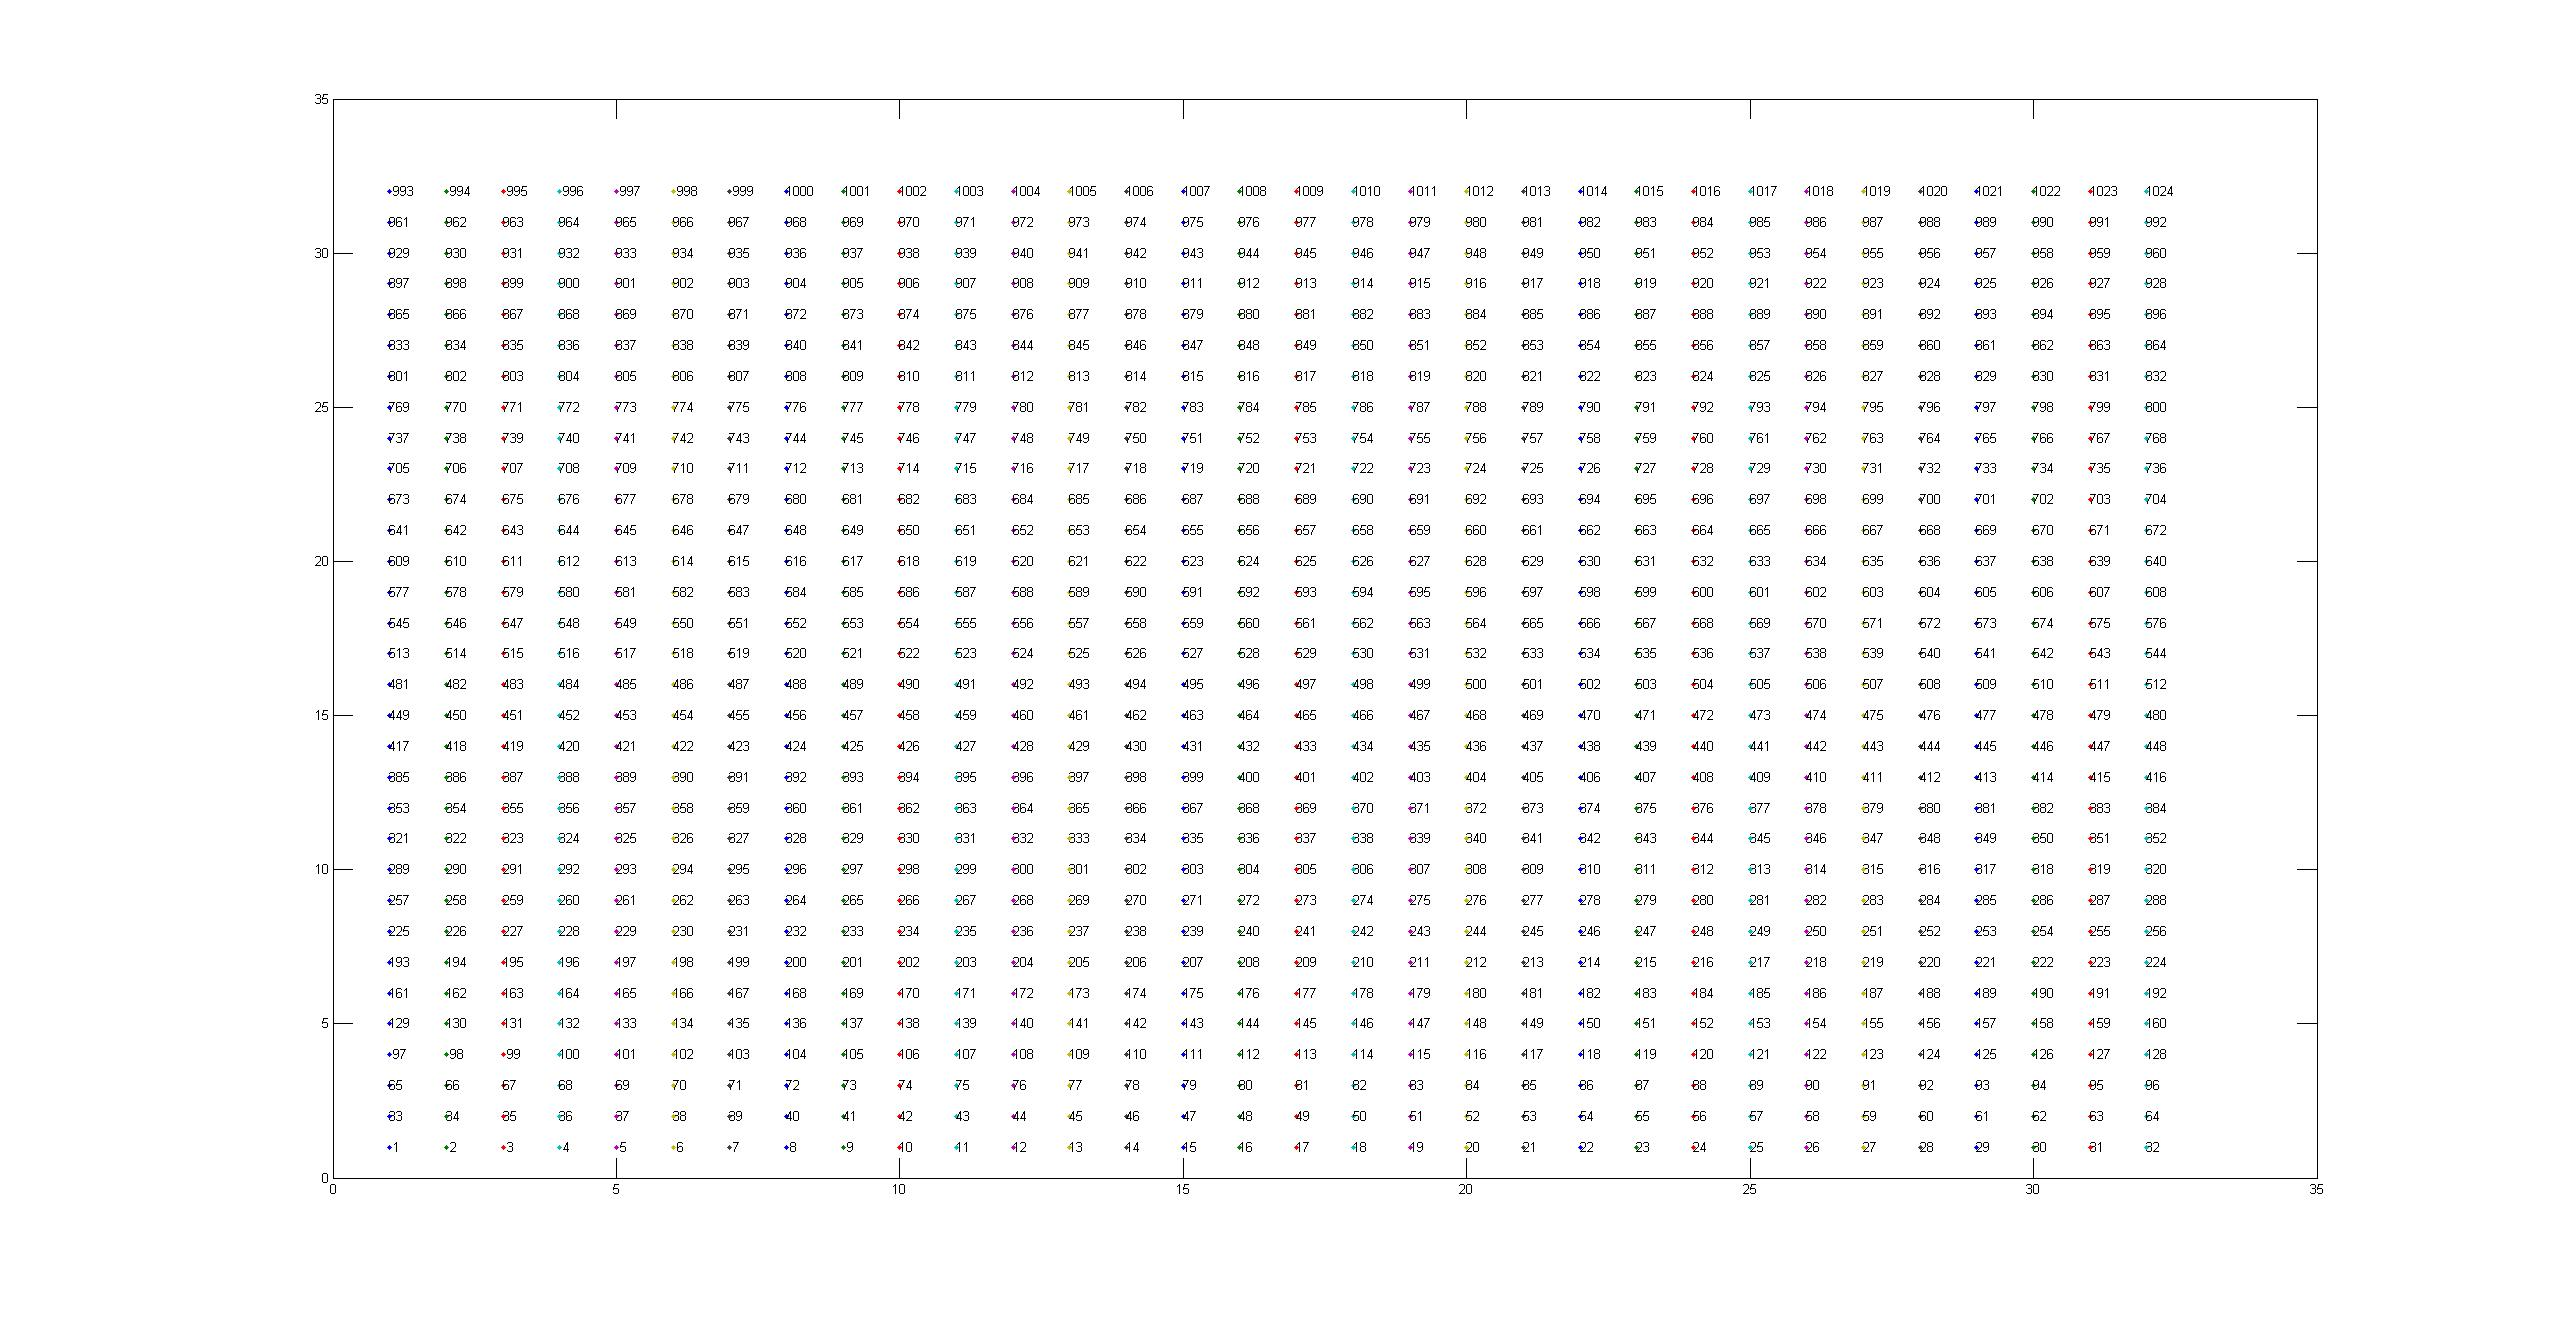
\includegraphics[width=1\textwidth]{29.jpg}
\caption{}
\end{figure}

\begin{figure}[!htbp]
\minipage{.5\textwidth}%
\centering
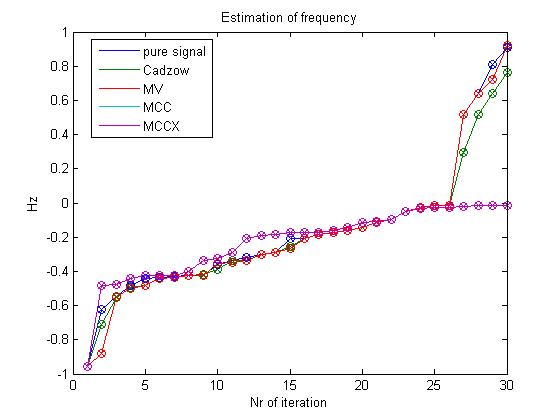
\includegraphics[width=1\textwidth]{31.jpg}
\subcaption{Frequency estimation}\label{LoveNadya1}
\endminipage\hfill
\minipage{.5\textwidth}%
\centering
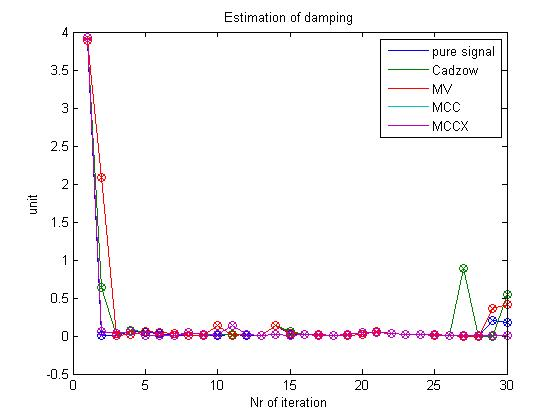
\includegraphics[width=1\textwidth]{32.jpg}
\subcaption{}
\endminipage\hfill
\minipage{.5\textwidth}%
\centering
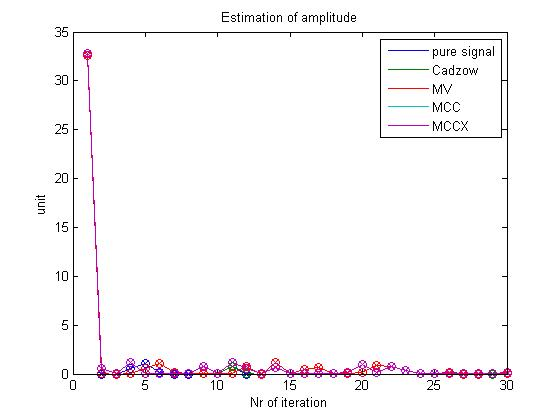
\includegraphics[width=1\textwidth]{33.jpg}
\subcaption{}
\endminipage\hfill
\minipage{.5\textwidth}%
\centering
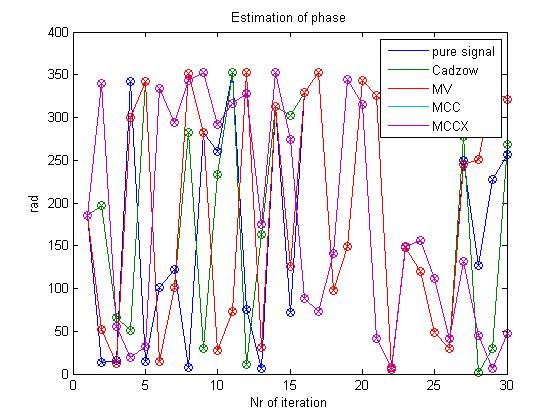
\includegraphics[width=1\textwidth]{34.jpg}
\subcaption{}
\endminipage\hfill
\caption{}
\end{figure}




\lstset{language=Matlab,%
    %basicstyle=\color{red},
    breaklines=true,%
    morekeywords={matlab2tikz},
    keywordstyle=\color{blue},%
    morekeywords=[2]{1}, keywordstyle=[2]{\color{black}},
    identifierstyle=\color{black},%
    stringstyle=\color{mylilas},
    commentstyle=\color{mygreen},%
    showstringspaces=false,%without this there will be a symbol in the places where there is a space
    numbers=left,%
    numberstyle={\tiny \color{black}},% size of the numbers
    numbersep=9pt, % this defines how far the numbers are from the text
    emph=[1]{for,end,break},emphstyle=[1]\color{red}, %some words to emphasise
    %emph=[2]{word1,word2}, emphstyle=[2]{style},    
}

\newpage
\section{Main code}
\lstinputlisting{Main_exercise_session.m}

%\subsection{Aid functions}
%\lstinputlisting{SignalDisplay.m}




\end{document}

